% Русская версия отчёта H3 (XeLaTeX)
\documentclass[11pt,a4paper]{article}
\usepackage{fontspec}
\setmainfont{cmunrm}[Extension=.otf,BoldFont=cmunbx,ItalicFont=cmunti,BoldItalicFont=cmunbi]
\setsansfont{cmunss}[Extension=.otf,BoldFont=cmunsx,ItalicFont=cmunsi,BoldItalicFont=cmunso]
\setmonofont{cmuntt}[Extension=.otf,BoldFont=cmuntb,ItalicFont=cmunit,BoldItalicFont=cmuntx]
\usepackage[english,russian]{babel}
\usepackage[margin=2.2cm]{geometry}
\usepackage{amsmath,amssymb,amsthm,mathtools,bm}
\usepackage{graphicx,booktabs,tabularx,xltabular,array,enumitem,xcolor}
\usepackage[most]{tcolorbox}
\usepackage{tikz}
\usetikzlibrary{arrows.meta,positioning}
\usepackage[colorlinks,linkcolor=blue!50!black,citecolor=green!35!black,urlcolor=blue!50!black]{hyperref}
\setlist{itemsep=1pt,topsep=2pt}
\setlength{\emergencystretch}{3em}
\numberwithin{equation}{section}
\newtheorem{theorem}{Теорема}[section]
\newtheorem{lemma}[theorem]{Лемма}
\newtheorem{proposition}[theorem]{Предложение}
\newtheorem{corollary}[theorem]{Следствие}
\theoremstyle{definition}
\newtheorem{definition}[theorem]{Определение}
\newtheorem{assumption}[theorem]{Предположение}
\theoremstyle{remark}
\newtheorem{remark}[theorem]{Замечание}
\newcommand{\E}{\mathbb E}\newcommand{\R}{\mathbb R}\newcommand{\Z}{\mathbb Z}\let\Prob\relax\newcommand{\Prob}{\mathbb P}
\newcommand{\norm}[1]{\lVert #1\rVert}\newcommand{\abs}[1]{\lvert #1\rvert}\newcommand{\ip}[2]{\langle #1,#2\rangle}
\newcommand{\Dmax}{\Delta_{\max}}\newcommand{\Dcp}{\Delta_{\rm cp}}\newcommand{\Dlow}{\Delta_{\rm low}}
\newcommand{\cN}{\mathcal N}\newcommand{\cA}{\mathcal A}\newcommand{\cG}{\mathcal G}\newcommand{\cF}{\mathcal F}
\newcommand{\Unif}{\mathrm{Unif}}\newcommand{\TV}{\mathrm{TV}}\newcommand{\BC}{\mathrm{BC}}\newcommand{\tmix}{t_{\rm mix}}
\newcommand{\Sph}{\mathbb S^{d-1}}\newcommand{\Ball}{\mathbb B}\newcommand{\iid}{\mathrm{iid}}
\newcommand{\wbar}{\bar\omega}\newcommand{\Atwo}{\cA^{\rm 2pt}_\gamma}
\definecolor{hl}{HTML}{2a78d6}
\tcbset{card/.style={breakable,colback=blue!2,colframe=blue!45!black,boxrule=0.6pt,arc=2pt,left=6pt,right=6pt,top=4pt,bottom=4pt,fonttitle=\bfseries}}

\title{\textbf{H3: независимые состояния ($\tau=1$)~---\\ двусторонняя оценка и закон $\sqrt T$\\ для двухточечных методов}\\[2pt]
\large Отчёт о локальном исследовании}
\author{}
\date{11~ноября 2026~г.}

\begin{document}
\maketitle
\tableofcontents

%==========================================================================================
\setcounter{section}{-1}
\section{Карточка-резюме}\label{sec:card}
\begin{tcolorbox}[card,title={H3 на одной странице}]
\textbf{Гипотеза.} Для независимых состояний ($\tau=1$) и $\gamma\le\gamma_\varepsilon$ порог шума для двухточечных методов радиуса $\gamma$ равен $\Theta(\varepsilon\gamma\sqrt T/(dR))$; существенный параметр шума~--- колебание (oscillation) $\delta$ на масштабе $\gamma$, а не $\Delta$.

\textbf{Вердикт: подтверждена в уточнённой форме.} Двусторонняя оценка доказана с явными константами для класса $\Atwo$ методов, которые видят только разности пары значений при радиусе $\le\gamma$ и выбирают направления из распределений, зафиксированных заранее (адаптивные центры, радиусы, шаги, усреднение, рестарты разрешены; класс содержит ZO-SGD), для выпуклых $M$-липшицевых $f$ при $\gamma\le\varepsilon/(4M)$; гладкий класс с $\varepsilon/(4M)<\gamma\le\sqrt{\varepsilon/L}$ нижней стороной не покрыт. Уточнения: (i)~нашей технике верхней оценки нужно распределение шума с конечной информацией Фишера (расстояние Хеллингера вместо KL); шум $\pm1$ с хэшированием, предложенный в формулировке гипотезы (утверждение H3.2), декодируется точно при $\Delta>2M\gamma$ на любой $f$ и при любом $\Delta$ на линейном гиперкубе (предл.~\ref{prop:pm1}, E3.5); является ли какой-либо двузначный шум трудным на уровнях, сохраняющих сложность, $\Delta\lesssim\sqrt C M\gamma/\sqrt d$, не решено; (ii)~ответ зависит от класса алгоритмов: для произвольных алгоритмов мы доказываем лишь $\Dlow\le\Dmax^E\le71\,\varepsilon\sqrt T/\sqrt d$ (предл.~\ref{prop:any}); цитируемые бандитные скорости после перенормировки на размах $f$ дают гарантию лишь при бюджетах $T\gtrsim C_bd^{k-1}T_0$, так что при бюджетах, сохраняющих сложность, $T\asymp CT_0$ они не превосходят двухточечные методы (следствие~\ref{cor:cross}); утверждение «в классе с фиксированным $\gamma$ бесселева часть блокирует бандитные методы» \emph{опровергнуто} сведением через усреднение по шару (предл.~\ref{prop:ballavg}); (iii)~обе стороны дословно верны с колебанием $\omega_\delta(2\gamma)/2$ вместо $\Delta$, а точной величиной является среднеквадратичное колебание $\wbar$; излом (knee) стоимости гладкого шума находится при $\ell\approx\gamma/\sqrt d$, а не при $\ell\approx\gamma$ (лемма~\ref{lem:sin}, E3.2).

\textbf{Главный результат (одна формула).} Для независимых одинаково распределённых состояний с произвольным начальным распределением (протокол H1), выпуклой $M$-липшицевой $f$ на $B_R$, $\gamma\le\varepsilon/(4M)$, $\varepsilon<MR/8$ и $T\ge 1+16d^2M^2R^2/((d-1)\varepsilon^2)$ раундов (по 2~вызова) в варианте «в~среднем»
\[
\frac{\varepsilon\gamma\sqrt{T-1}}{4\,dR}\ \le\ \frac{\gamma}{d}\Big(\frac{\varepsilon\sqrt{T-1}}{2R}-\frac{dM}{\sqrt{d-1}}\Big)\ \le\ \Dmax^{E,\mathrm{2pt},\gamma}(\varepsilon;\iid;T)\ \le\ 32\pi\,\frac{\varepsilon\gamma\sqrt T}{dR}
\qquad(\text{теор.~\ref{thm:main}}).
\]
Нижняя сторона~--- ZO-SGD с пакетом размера 1, простаивающий в раунде~1 (состояние раунда 1 имеет произвольное начальное распределение; при стационарном старте $T-1$ заменяется на $T$); никакого другого прогрева нет. Верхняя сторона~--- один пример (линейные $f_v$, негладкий клеточный шум с плотностью $\cos^2(\pi t/2)$), лежащий в классе всех радиусов и удовлетворяющий обоим прочтениям (2). Следствия: в варианте «в~среднем» $\Dcp^{E}(24)\ge1.034\,M\gamma/\sqrt d$ при $\tau=1$ (в H1 было $C=261$, $M\gamma/\sqrt{2d+5}$); отдельно верхняя сторона даёт $\Dcp^{E,\mathrm{2pt},\gamma}(C)\le32\pi\sqrt C\,M\gamma/\sqrt d$, что закрывает H1.5d для $\tau=1$ и $\Atwo$.

\textbf{Что это означает для задачи.} Случай $\tau=1$~--- теорема, а не эвристика: первая ветвь H2 при $\tau=1$ верна с обеих сторон \emph{для класса $\Atwo$}; верхняя сторона ожидаемой картины, $\Dcp\lesssim M\gamma/\sqrt d$ (H1.5d), доказана для этого класса. Для произвольных точек запроса наши оценки оставляют разрыв $\asymp\sqrt d\,MR/\varepsilon$, поэтому ответ зависит от того, к какому классу алгоритмов относится $\Dmax$; для произвольных алгоритмов он остаётся открытым (\S\ref{sec:contrib}).

\textbf{Численные эксперименты} (по 5~запусков). E3.1 (логистическая регрессия и $\ell_1$, $d\in\{20,80\}$, $T\le10^6$): совмещение (collapse) по $\Delta/\sqrt T$ подтверждено на подмножествах с продвижением (progress) четырёх основных задач ($a=0.49$--$0.52$, каждый ДИ содержит $\frac12$); на всех точках с преобладанием шума $a=0.50$--$0.56$, и для обеих задач с $d=80$ ДИ исключает $\frac12$ (на $\le0.03$), что удовлетворяет критерию «$a\ne\frac12$», зафиксированному в формулировке гипотезы до этого исследования, но не критерию отчёта ($a\notin[0.4,0.6]$); ошибки $\le0.25$ от оценки теоремы. Вариант чувствительности с шумом $\pm1$ удовлетворяет критерию опровержения отчёта ($a=0.67$); на уровнях с тем же $\wbar$, что и в запусках с бета-шумом, подгонка по всем точкам даёт $a=0.52$, но подмножество с продвижением ($29$~точек) даёт $a=0.63\ [0.52,0.77]$, так что насыщение объясняет большую часть аномалии, но не всю. E3.2: $\E\|n\|^2\propto1-\Phi_d(2\gamma/\ell)$ с точностью до $0.6\%$; в оптимизации стоимость при $\ell=\gamma$ равна $0.18$ ($d=20$) и $0.07$ ($d=80$), а не $1$, как предсказывает $\min\{1,(\gamma/\ell)^2\}$; согласие с $1-\Phi_d$ с точностью до множителя~2 выполнено для $d=20$ и нарушено для $d=80$ (насыщенный дизайн). E3.4 (только проверка на здравый смысл, sanity check): ZO-SGD ни разу не оказывается лучше оценки Ассуада на трудном примере. E3.5: декодированный шум $\pm1$ воспроизводит запуск без шума с точностью до $10^{-16}$. E3.3 не запускался (вместо него аналитическое сравнение и план).

\end{tcolorbox}

%==========================================================================================
\section{Место в глобальной задаче}\label{sec:place}
\textbf{Закрываемое узкое место.} Верхняя сторона ожидаемой картины из постановки задачи (её \S3, абзац «Ожидаемая картина»; эвристика $\Delta\lesssim M\gamma/\sqrt d$ сформулирована в её \S1, в абзаце после условия ортогональности): $M\gamma/\sqrt d$ была эвристикой по дисперсии без верхней оценки. H1 доказала её нижнюю сторону ($\Dcp\ge M\gamma/\sqrt{2d+8\tau-3}$) и оставила верхнюю сторону как H1.5d. H3 доказывает обе стороны при $\tau=1$ и фиксирует класс алгоритмов, в котором утверждение верно. Она также касается выбора трудной конструкции: двузначное распределение, предложенное в формулировке гипотезы (утверждение H3.2), декодируемо (при $\Delta>2M\gamma$ на любой $f$, при любом $\Delta$ на линейном гиперкубе), и наша техника верхней оценки использует вместо него распределение с конечной информацией Фишера; \emph{необходимо} ли такое распределение, не показано.

\textbf{Зависит от.} Отчёт H1: опр.~4.19 (протокол, $\Dmax$), лемма~4.1 (перестановка $\E_\pi$, $\E_e$), лемма~4.3 (тождество Стокса для шара), предл.~4.4 (сведение к $m$), лемма~4.14(a) (оценка Пуанкаре $\E\|g_f\|^2\le d^2M^2/(d-1)$), следствие~4.23 (переход от варианта «в~среднем» к варианту «по~вероятности»). \textbf{Используется в.} H2 (её первая ветвь при $\tau=1$ с обеих сторон, для $\Atwo$), H5 (техника верхней оценки для ограниченного шума), H4 (базовый случай $\tau=1$), H7/H10 (округление как шум с $\tau=1$: форма через колебание, предл.~\ref{prop:round}).

\begin{figure}[h]\centering
\begin{tikzpicture}[node distance=7mm and 9mm, every node/.style={font=\small},
  h/.style={draw,rounded corners=2pt,minimum width=12mm,minimum height=6mm,fill=gray!6},
  done/.style={h,fill=green!8,draw=green!45!black},
  cur/.style={h,fill=hl!18,draw=hl,line width=1.1pt},
  ar/.style={-{Stealth[length=2mm]},gray!70!black}, dar/.style={ar,dashed}]
\node[done] (H1) {\textbf{H1} определение};
\node[cur,below left=9mm and 22mm of H1] (H3) {\textbf{H3} $\tau{=}1$};
\node[h,right=6mm of H3] (H4) {H4 сведение};
\node[h,right=6mm of H4] (H5) {H5 трудн.\ констр.};
\node[h,right=6mm of H5] (H6) {H6 переход по $\gamma$};
\node[h,below=12mm of H4] (H2) {\textbf{H2} $\Dmax(T,\tau)$};
\node[h,right=14mm of H2] (H9) {H9 $T_{\rm eff}$};
\node[h,left=14mm of H2] (H8) {H8 ленивая цепь};
\node[h,below=8mm of H8] (H7) {H7 самодизеринг};
\node[h,below=8mm of H2] (H10) {H10 общий дизеринг};
\draw[ar] (H1) -- (H3); \draw[ar] (H1) -- (H4); \draw[ar] (H1) -- (H5); \draw[ar] (H1) -- (H6);
\draw[ar,line width=1pt,hl] (H3) -- (H2); \draw[ar,line width=1pt,hl] (H3) -- (H5); \draw[ar,line width=1pt,hl] (H3.south) to[out=-110,in=170] (H10.west);
\draw[ar] (H4) -- (H2); \draw[ar] (H5) -- (H2);
\draw[ar] (H2) -- (H8); \draw[ar] (H2) -- (H9); \draw[ar] (H7) -- (H8); \draw[dar] (H6) -- (H2);
\node[font=\scriptsize,text=hl,align=left,left=3mm of H3] {обе стороны первой ветви\\H2 при $\tau{=}1$ для $\Atwo$;\\техника Хеллингера $\to$ H5;\\округление как шум\\с $\tau{=}1$ $\to$ H7/H10};
\end{tikzpicture}
\caption{Зависимости между H1--H10 (стрелки: «используется в»). H3 выделена; H1 (зелёная) проверена. Толстые синие стрелки: что даёт H3.}
\label{fig:diagram}
\end{figure}

%==========================================================================================
\section{Постановка и мотивация}\label{sec:statement}
\subsection{Определения}
Обозначения~--- из глобального контекста и H1: $B_r=\{x:\norm x\le r\}$, $\Ball=B_1$, $e\sim\Unif(\Sph)$, $u,w\sim\Unif(\Ball)$, $d\ge2$; $f$ выпукла и $M$-липшицева на $B_R$; $f_\gamma(x)=\E_uf(x+\gamma u)$; $T_0=dM^2R^2/\varepsilon^2$. Протокол~--- опр.~4.19 из H1 с $q=2$: раунды $k=1,\dots,T$, один шаг цепи за раунд, экзогенная цепь, оба запроса раунда в одном и том же состоянии.

\begin{definition}[Независимые состояния]\label{def:iid}
$\cN_\iid(\Delta;\Gamma)$~--- множество экземпляров шума из H1, опр.~4.19(i), ядро которых равно $P(s,\cdot)=\pi$ для каждого $s$. Как и в H1, начальное распределение $\nu$ состояния $s_1$ произвольно; далее $s_2,s_3,\dots$ независимы, одинаково распределены $\sim\pi$ и не зависят от $s_1$, а $s_1\sim\nu$ («стационарный старт» означает $\nu=\pi$, т.\,е.\ все состояния независимы и одинаково распределены $\sim\pi$). Экземпляр состоит из стандартного борелевского пространства $S$, совместно борелевской функции $\delta:\R^d\times S\to[-\Delta,\Delta]$ и условия (2) для почти всех $x\in B_{R-\gamma'}$ и каждого $\gamma'\in\Gamma$. $\Gamma=(0,\gamma_0]$~--- рекомендуемый класс всех радиусов (эквивалентно $\E_\pi\delta(x,\cdot)=c$ почти всюду, H1 теор.~4.10); $\Gamma=\{\gamma\}$~--- вариант с фиксированным радиусом. «$\tau=1$» в этом отчёте означает $\cN_\iid$; этот класс содержится в классе $\tmix\le1$ и, следовательно, в каждом $\cN(\Delta,\tau)$.
\end{definition}

\begin{definition}[Двухточечные методы радиуса $\gamma$: класс $\Atwo$]\label{def:class}
Алгоритм с $T$ раундами принадлежит $\Atwo$, если у него есть внутренняя случайность $\xi_0$ (выбирается один раз) и свежие независимые равномерные величины $\zeta_1,\zeta_2,\dots$, и в раунде $t$ он:
(a)~выбирает направление $e_t=E_t(\xi_0,\zeta_t)\in\Sph$, так что распределение $\mu_t(\xi_0)$ направления $e_t$ зависит только от $t$ и $\xi_0$, но не от прошлых наблюдений;
(b)~выбирает центр и радиус $(y_t,\gamma_t)=Y_t(\xi_0,\zeta_t,e_t,H_{t-1})$ с $\gamma_t\in(0,\gamma]$ и $y_t\pm\gamma_te_t\in B_R$, где $H_{t-1}=(e_s,y_s,\gamma_s,D_s)_{s<t}$;
(c)~наблюдает только разность $D_t=O(y_t+\gamma_te_t,s_t)-O(y_t-\gamma_te_t,s_t)$.
После $T$ раундов он выдаёт $\hat x=X(\xi_0,H_T)\in B_R$ (все отображения борелевские). $\Dmax^{\mathrm{2pt},\gamma}$~--- это $\Dmax$ из H1, опр.~4.19, в котором супремум по алгоритмам ограничен классом $\Atwo$; верхний индекс $E$ обозначает вариант «в~среднем».
\end{definition}
$\Atwo$ содержит ZO-SGD с любым правилом выбора шага, пакетированием, усреднением итераций, рестартами, импульсом (momentum) и случайными центрами запросов; он исключает методы, читающие отдельные значения (например, сравнивающие $O$ в далёких точках из разных раундов), адаптивный выбор распределения направлений (например, адаптивный выбор координат) и радиусы больше $\gamma$.

\begin{definition}[Колебание]\label{def:osc}
$\omega_\delta(2\gamma)=\sup_s\sup_{\norm{y-z}\le2\gamma}\abs{\delta(y,s)-\delta(z,s)}\le2\Delta$ (как в формулировке гипотезы), и среднеквадратичное колебание пары $\wbar(y)^2=\E_{s\sim\pi}\E_e\big[(\delta(y+\gamma e,s)-\delta(y-\gamma e,s))^2\big]$, $\wbar=\sup_{y\in B_{R-\gamma}}\wbar(y)\le\omega_\delta(2\gamma)$.
\end{definition}

\subsection{Утверждения}
\begin{center}\small
\begin{tabularx}{\textwidth}{@{}lX@{}}
\toprule
H3.1 & Нижняя оценка: ZO-SGD (пакет размера 1, радиус $\gamma$, холостой раунд~1) имеет точность $\varepsilon$ в среднем при каждом $\Delta\le\Dlow(T)=\frac\gamma d\big(\frac{\varepsilon\sqrt{T-1}}{2R}-\frac{dM}{\sqrt{d-1}}\big)_+$; $\Dcp^E(24)\ge M\gamma/\sqrt d$; при $\xi\equiv0$ по порядку восстанавливается эвристический порог $M\gamma/\sqrt d$ ожидаемой картины (неформальная проверка согласованности). \\
H3.2 & Верхняя оценка для $\Atwo$: $\Dmax^{E,\mathrm{2pt},\gamma}\le32\pi\,\varepsilon\gamma\sqrt T/(dR)$ через гиперкуб линейных функций и негладкий клеточный шум; клеточный шум $\pm1$ такой оценки \emph{не} даёт. \\
H3.3 & Развилка: (a)~любой алгоритм, $\Dmax^E\le16\sqrt2\pi\,\varepsilon\sqrt T/\sqrt d$; (b)~где бандитные скорости лучше двухточечной формулы ($MR/\varepsilon\gtrsim\sqrt d$ для скоростей $d^3$ и только при бюджетах $T\gtrsim d^{k-1}T_0$)~--- при условии справедливости цитируемых результатов; (c)~в классе с фиксированным $\gamma$ бесселева часть \emph{не} блокирует бандитные методы. \\
H3.4 & Колебание: шумовая часть оценки $\le d\,\omega_\delta(2\gamma)/(2\gamma)$; H3.1--H3.2 верны с $\omega_\delta/2$ (и $\wbar/2$) вместо $\Delta$; $\Lambda$-липшицев шум стоит $M\to M+\Lambda$; для округления $\omega_\delta\le u$, $\wbar\le u/2$, совпадение (tie) $\Leftrightarrow$ сигнал стёрт. \\
H3.5 & Численные эксперименты: E3.1~--- совмещение по $\Delta/\sqrt T$; E3.2~--- стоимость в зависимости от масштаба $\ell$; E3.3 (не запускался); E3.4~--- трудный пример (проверка на здравый смысл); E3.5~--- декодирование шума $\pm1$. \\
\bottomrule
\end{tabularx}
\end{center}
Формулировка гипотезы, включая цитируемые в этом отчёте предсказания и критерии опровержения, была зафиксирована до исследования.

\subsection{Почему это стоит проверять; следствия}
$\tau=1$~--- единственный случай основной формулы H2, который можно полностью решить уже сейчас. Если бы закон $\sqrt T$ не выполнялся для независимых состояний, H2 была бы неверна. Если он выполняется, случай $\tau=1$ становится теоремой с константами и классом методов, в котором она верна, а остальная часть H2 становится вопросом о том, как входит $\tau$. Важнее всего верхняя сторона: это первое строгое утверждение о том, что ортогональность \emph{не может} дать больше, чем $\sqrt T$, для двухточечных методов, т.\,е.\ что ожидаемая картина $M\gamma/\sqrt d$ при $T\asymp T_0$~--- настоящий порог, а не артефакт анализа дисперсии. Если бы, напротив, какой-то двухточечный метод выдерживал больше, ожидаемая картина была бы лишь нижней оценкой, и H2 потребовалась бы другая первая ветвь.

%==========================================================================================
\section{Что известно}\label{sec:known}
\begin{center}\small
\begin{tabularx}{\textwidth}{@{}p{2.6cm}Xp{2.5cm}@{}}
\toprule
Пункт & Утверждение в том виде, в каком оно используется здесь & Статус здесь\\
\midrule
Двухточечные скорости и минимаксные нижние оценки & Duchi, Jordan, Wainwright, Wibisono, \emph{Optimal rates for zero-order convex optimization: the power of two function evaluations}, arXiv:1312.2139v2: следствие~1 (скорость $RG\sqrt d/\sqrt k$ при направлениях на сфере), предл.~1 (нижняя оценка $\frac1{12}(1-\frac1q)\frac{GR}{\sqrt k}\min\{d^{1-1/q},k^{1-1/q}\}$ для линейных \emph{стохастических} функционалов $F(\theta;X)=\ip\theta X$ с гауссовским $X$; о детерминированной $f$ при $\Delta=0$ оно ничего не говорит), лемма~6 (разделение на шарах $\ell_q$), лемма~7 (цепное правило для KL при адаптивных парах), предл.~3 (нижняя оценка для одного вычисления $\frac14\min\{d\sigma/\sqrt k,\dots\}$). & используется как образец; шаг разделения передоказан (лемма~\ref{lem:assouad}); KL заменено расстоянием Хеллингера (для ограниченного шума KL бесконечно) \\
Ассуад / Ле Кам & B.~Yu, \emph{Assouad, Fano, and Le Cam} (1997); неравенство Ле Кама $P(A)+Q(A^c)\ge1-\TV(P,Q)$. & используется, доказательство приведено \\
Расстояние Хеллингера для семейств сдвигов & $H^2(p_b,p)\le b^2I(p)/4$ для абсолютно непрерывной $\sqrt p$ с информацией Фишера $I(p)$ (например, Ибрагимов--Хасьминский, \emph{Statistical Estimation}, гл.~I); неравенство обработки данных для $f$-дивергенций; $\TV\le\sqrt{1-\BC^2}$. & передоказано (леммы~\ref{lem:hell}, \ref{lem:seq}); проверено численно (V3, V4, V7) \\
Минимальная информация Фишера на $[-1,1]$ & $\cos^2(\pi t/2)$ имеет $I=\pi^2$~--- минимум по плотностям на $[-1,1]$ (классический факт; для корректности не нужен). & $I=\pi^2$ проверено символьно (V1); минимальность не используется \\
Враждебный порог & Pasechnyuk-Vilensky et al.\ arXiv:2306.16371v5, теор.~III.1, предл.~IV.1 (в формулировке H1 \S3). & в доказательствах не используется \\
Одноточечные (бандитные) методы & Lattimore--Gy\"orgy, COLT 2023, arXiv:2302.05371; Fokkema et al., COLT 2024, arXiv:2406.06506: выпуклая одноточечная оптимизация с верхними скоростями $d^3$--$d^{3.5}\varepsilon^{-2}$ (с точностью до логарифмов), без масштаба шума. Как указано в этих работах, постановка~--- потери со значениями в $[0,1]$ и условно субгауссовский шум постоянного масштаба. Номера теорем мы не приводим и формулировки теорем, постановки, константы и логарифмы \emph{не} перепроверяли. & используется только в условном следствии~\ref{cor:cross}, с явно указанным размахом (предположение~(B)); помечено \\
Липшицева систематическая часть & Loginov et al.\ arXiv:2610.05517 рассматривают систематическую липшицеву компоненту (формулировка не перепроверялась). & только замечание \\
Получено нами ранее & Отчёт H1: леммы 4.1, 4.3, 4.14(a); предл.~4.4; теор.~4.15 и следствие~4.17 (нижняя половина H2 с прогревом, $V=2d^2M^2/(d-1)+(2d+8\tau-3)d\Delta^2/\gamma^2$); следствие~4.23. Эвристика по дисперсии, на которой основана ожидаемая картина: порог $M\gamma/\sqrt d$ (\S\ref{sec:place}). & используется \\
Новое в этом отчёте & Лемма~\ref{lem:mom}--предл.~\ref{prop:round}; эксперименты E3.1, E3.2, E3.4, E3.5; проверки V1--V17. & \\
\bottomrule
\end{tabularx}
\end{center}
%==========================================================================================
\section{Теория}\label{sec:theory}
Всюду $f$ выпукла и $M$-липшицева на $B_R$, $f^*=\min_{B_R}f$, $d\ge2$, $0<\gamma<R$, протокол~--- H1 опр.~4.19 с $q=2$, и цепь имеет независимые одинаково распределённые состояния (опр.~\ref{def:iid}).

\subsection{H3.1: нижняя оценка (алгоритм)}\label{sec:lower}
\emph{Почему это должно быть верно и в чём трудность.} При независимых одинаково распределённых состояниях каждый раунд~--- свежая независимая реализация оценки со средним $\nabla f_\gamma$ (H1 предл.~4.4: смещение при фиксированном состоянии усредняется по $\pi$), так что метод~--- обычный SGD с ограниченным вторым моментом, и вся работа состоит в том, чтобы получить второй момент с правильными константами. В H1 корреляция между состояниями вынуждала делать прогрев и давала оценку $(2d+8\tau-3)d\Delta^2/\gamma^2$; для независимых состояний ни то ни другое не нужно, и шум входит только через среднеквадратичное колебание пары. Две тонкости. Прочтение (2) «почти всюду»: центр запроса должен избегать множества меры нуль, что обеспечивает случайный центр радиуса $\rho>0$. Начальное распределение: протокол разрешает $s_1$ иметь произвольное распределение $\nu$, а (2)~--- среднее по $\pi$, поэтому оценка, построенная в раунде~1, может быть смещена; поэтому метод простаивает в раунде~1 (или предполагается, что цепь стартует из $\pi$).

\begin{lemma}[Одно состояние, одно направление]\label{lem:mom}
Пусть $y\in B_{R-\gamma}$~--- точка, в которой (2) выполнено при радиусе $\gamma$, $e\sim\Unif(\Sph)$ и $s\sim\pi$ независимы и $Y=\frac d{2\gamma}\big(O(y+\gamma e,s)-O(y-\gamma e,s)\big)e$. Тогда
\[
\text{(a)}\ \ \E Y=\nabla f_\gamma(y),\qquad\text{(b)}\ \ \big(\E\norm Y^2\big)^{1/2}\le\frac{dM}{\sqrt{d-1}}+\frac{d\,\wbar(y)}{2\gamma}\le\frac{dM}{\sqrt{d-1}}+\frac{d\,\omega_\delta(2\gamma)}{2\gamma}\le \frac{dM}{\sqrt{d-1}}+\frac{d\Delta}{\gamma}.
\]
\end{lemma}
\begin{proof}
Запишем $Y=g_f+n$, где $g_f=\frac d{2\gamma}(f(y+\gamma e)-f(y-\gamma e))e$ и $n=\frac d{2\gamma}(\delta(y+\gamma e,s)-\delta(y-\gamma e,s))e$.
(a)~$\E g_f=\frac d\gamma\E[f(y+\gamma e)e]=\nabla f_\gamma(y)$ в силу $e\mapsto-e$ и тождества Стокса для шара для непрерывной $f$ (H1 лемма~4.3(b)). В силу $e\mapsto-e$ и теоремы Фубини (H1 лемма~4.1; $\delta$ совместно борелевская и ограниченная) $\E n=\frac d\gamma\E_{s\sim\pi}\E_e[\delta(y+\gamma e,s)e]=0$ по (2) в точке $y$.
(b)~Неравенство Минковского в $L^2$: $(\E\norm Y^2)^{1/2}\le(\E\norm{g_f}^2)^{1/2}+(\E\norm n^2)^{1/2}$. Первое слагаемое $\le dM/\sqrt{d-1}$ по H1 лемме~4.14(a) (неравенство Пуанкаре на $\Sph$, применённое к $e\mapsto f(y+\gamma e)$; численно перепроверено в V11). Поскольку $\norm e=1$, $\E\norm n^2=\frac{d^2}{4\gamma^2}\E(\delta(y+\gamma e,s)-\delta(y-\gamma e,s))^2=\frac{d^2\wbar(y)^2}{4\gamma^2}$, и $\wbar(y)\le\omega_\delta(2\gamma)\le2\Delta$.
\end{proof}

\paragraph{Алгоритм ZO$(T,\gamma,\rho,\eta;t_0)$.} $t_0\in\{0,1\}$~--- число холостых раундов в начале, $N=T-t_0$~--- число шагов, $R'=R-\gamma-\rho>0$, $x_1=0$. Раунды $1,\dots,t_0$: без запроса. Шаг $i=1,\dots,N$, выполняемый в раунде $t=t_0+i$: выбрать $w_i\sim\Unif(\Ball)$, $e_i\sim\Unif(\Sph)$, положить $y_i=x_i+\rho w_i$, запросить $y_i\pm\gamma e_i$ в состоянии $s_t$, построить $Y_i=\frac d{2\gamma}D_ie_i$ и $x_{i+1}=\Pi_{B_{R'}}(x_i-\eta Y_i)$. Выход: $\bar x=\frac1N\sum_{i\le N}x_i$. Алгоритм принадлежит $\Atwo$ (распределение направлений~--- $\Unif(\Sph)$; $y_i$ использует свежую случайность и историю; холостой раунд~--- это раунд с неинформативным запросом, например с игнорируемым $D_t$).

\begin{theorem}[Нижняя оценка с явными константами]\label{thm:lower}
Пусть $\delta\in\cN_\iid(\Delta;\Gamma)$, $\gamma\in\Gamma$, и пусть $\rho\ge0$, $\gamma+\rho<R$, причём $\rho=0$ допускается, если (2) выполнено при радиусе $\gamma$ для каждого $x\in B_{R-\gamma}$, и $\rho>0$ в противном случае. Поточечное условие выполнено, в частности, если $\delta(\cdot,s)\in\cG_\gamma$ для каждого $s$: по H1 лемме~4.3(b) каждая $S_{\delta(\cdot,s)}(x)=\frac d\gamma\E_e[\delta(x+\gamma e,s)e]$ непрерывна по $x$ и ограничена величиной $\sqrt d\Delta/\gamma$, так что $S_m=\E_\pi S_{\delta(\cdot,s)}$ (H1 лемма~4.1) непрерывна по теореме о мажорированной сходимости; она обращается в нуль почти всюду в силу (2), а значит, всюду. Пусть $t_0=1$ (произвольное начальное распределение) или $t_0=0$ (стационарный старт, $s_1\sim\pi$), $N=T-t_0\ge1$, и положим
\[
G=\frac{dM}{\sqrt{d-1}}+\frac{d\,\wbar}{2\gamma},\qquad \eta=\frac{R}{G\sqrt N}.
\]
Тогда ZO$(T,\gamma,\rho,\eta;t_0)$ использует $T$ раундов ($2N$ вызовов) и
\[
\E f(\bar x)-f^*\ \le\ \frac{RG}{\sqrt{T-t_0}}+2M(\gamma+\rho).
\]
\end{theorem}
\begin{proof}
Пусть $F(x)=\E_{w,u}f(x+\rho w+\gamma u)$ на $B_{R'}$. $F$ выпукла и $M$-липшицева, $f\le F\le f+M(\gamma+\rho)$ (неравенство Йенсена, так как $\E[\rho w+\gamma u]=0$; липшицевость), и $\nabla F(x)=\E_w\nabla f_\gamma(x+\rho w)$ ($f_\gamma\in C^1$ с $\norm{\nabla f_\gamma}\le M$, H1 лемма~4.3(b); мажорированная сходимость). Пусть $\cF_{i-1}$ порождена всем, что было до шага $i$ (включая $s_1,\dots,s_{t_0+i-1}$). Шаг $i$ использует состояние $s_{t_0+i}$. Если $t_0=1$, то $t_0+i\ge2$, и $s_{t_0+i}\sim\pi$ не зависит от $\cF_{i-1}$ и от $(w_i,e_i)$, поскольку из $P(s,\cdot)=\pi$ следует, что $s_2,s_3,\dots$ независимы, одинаково распределены $\sim\pi$ и не зависят от $s_1$ при любом начальном распределении, а цепь экзогенна. Если $t_0=0$, то же верно для $i=1$, так как $s_1\sim\pi$ по предположению. (Независимости $s_1$ от алгоритма недостаточно, если $s_1\not\sim\pi$: лемме~\ref{lem:mom}(a) нужно $s\sim\pi$; см.\ замечание~\ref{rem:lower}(vi).) Если $\rho>0$, то $y_i$ имеет плотность при условии $\cF_{i-1}$, так что (2) выполнено в $y_i$ почти наверное; если $\rho=0$, то оно выполнено всюду по предположению. По лемме~\ref{lem:mom} $\E[Y_i\mid\cF_{i-1}]=\E_w\nabla f_\gamma(x_i+\rho w)=\nabla F(x_i)$ и $\E[\norm{Y_i}^2\mid\cF_{i-1}]\le G^2$.
Пусть $x'=\Pi_{B_{R'}}x^*$, так что $\norm{x_1-x'}\le R'\le R$ и $\norm{x'-x^*}\le\gamma+\rho$. Нерастягиваемость проекции даёт $\norm{x_{i+1}-x'}^2\le\norm{x_i-x'}^2-2\eta\ip{Y_i}{x_i-x'}+\eta^2\norm{Y_i}^2$. Беря математические ожидания и пользуясь выпуклостью, получаем $2\eta\E[F(x_i)-F(x')]\le2\eta\E\ip{\nabla F(x_i)}{x_i-x'}\le\E\norm{x_i-x'}^2-\E\norm{x_{i+1}-x'}^2+\eta^2G^2$. Суммируя по $i\le N$, деля на $2\eta N$ и применяя неравенство Йенсена,
$\E F(\bar x)-F(x')\le\frac{R^2}{2\eta N}+\frac{\eta G^2}2=\frac{RG}{\sqrt N}$.
Наконец, $f(\bar x)\le F(\bar x)$ и $F(x')\le f(x')+M(\gamma+\rho)\le f^*+2M(\gamma+\rho)$.
\end{proof}

\begin{corollary}[Допустимый уровень]\label{cor:lower}
Пусть $\gamma+\rho\le\varepsilon/(4M)$ с $\rho$ как в теор.~\ref{thm:lower}, и пусть начальное распределение произвольно ($t_0=1$). Тогда каждый экземпляр с $\wbar/2\le\Dlow(T)$, в частности каждая $\delta\in\cN_\iid(\Delta;\Gamma)$ с $\Delta\le\Dlow(T)$, решается с точностью $\varepsilon$ в среднем за $T$ раундов, где
\begin{equation}\label{eq:Dlow}
\Dlow(T)=\frac\gamma d\Big(\frac{\varepsilon\sqrt{T-1}}{2R}-\frac{dM}{\sqrt{d-1}}\Big)_+ .
\end{equation}
(При стационарном старте $t_0=0$, и $T-1$ можно всюду ниже заменить на $T$.) Следовательно, $\Dmax^{E,\mathrm{2pt},\gamma}(\varepsilon;\iid;T)\ge\Dlow(T)$, и:
\begin{enumerate}[label=(\alph*)]
\item если $T\ge1+16d^2M^2R^2/((d-1)\varepsilon^2)$, то $\Dlow(T)\ge\varepsilon\gamma\sqrt{T-1}/(4dR)$;
\item (вариант «в~среднем») если $\varepsilon<MR/8$, то для каждого $d\ge2$
\[\Dcp^{E}(24)\ge\Dcp^{E,\mathrm{2pt},\gamma}(24)\ge\Dlow(24T_0)=\frac{M\gamma}{\sqrt d}\Big(\sqrt{6(1-1/(24T_0))}-\sqrt{d/(d-1)}\Big)\ge1.034\,\frac{M\gamma}{\sqrt d}\] (V15; без холостого раунда множитель равен $\sqrt6-\sqrt2=1.035$, V9). В варианте «по~вероятности» общего блока та же оценка верна при $C=24/\beta^2$: $\Dcp(24/\beta^2)\ge1.034\,M\gamma/\sqrt d$ при $\gamma+\rho\le\beta\varepsilon/(4M)$ и $\beta\varepsilon<MR/8$ (в силу (d); ср.\ H1 следствие~4.23(c));
\item в форме, данной в формулировке гипотезы: $G^2\le2d^2M^2/(d-1)+2d^2\Delta^2/\gamma^2\le4dM^2+2d^2\Delta^2/\gamma^2$, так что «$G^2\le c(dM^2+d^2\Delta^2/\gamma^2)$» выполнено с $c=4$, а условие $RG/\sqrt{T-1}\le\varepsilon/2$ следует из $\Delta\le\frac\gamma d\sqrt{(T-1)\varepsilon^2/(8R^2)-2dM^2}$~--- немного более слабого варианта \eqref{eq:Dlow};
\item (вариант «по~вероятности») $\Dmax(\varepsilon,\beta;\iid;T)\ge\Dlow(T)|_{\varepsilon\to\beta\varepsilon}$ по неравенству Маркова (H1 следствие~4.23), при $\gamma+\rho\le\beta\varepsilon/(4M)$.
\end{enumerate}
\end{corollary}
\begin{proof}
По теор.~\ref{thm:lower} с $t_0=1$ $\E f(\bar x)-f^*\le RG/\sqrt{T-1}+\varepsilon/2$, и $RG/\sqrt{T-1}\le\varepsilon/2$ тогда и только тогда, когда $\frac{d\wbar}{2\gamma}\le\frac{\varepsilon\sqrt{T-1}}{2R}-\frac{dM}{\sqrt{d-1}}$, т.\,е.\ $\wbar/2\le\Dlow(T)$; при этом $\wbar\le2\Delta$. (a)~$\frac{\varepsilon\sqrt{T-1}}{4R}\ge\frac{dM}{\sqrt{d-1}}$ при условии на $T$. (b)~ZO принадлежит $\Atwo$, поэтому $\Dcp^E\ge\Dcp^{E,\mathrm{2pt},\gamma}$. При $T=24T_0$ $\frac{\varepsilon\sqrt{T-1}}{2R}=\sqrt dM\sqrt{6(1-1/(24T_0))}$. Множитель $\sqrt{6(1-1/(24T_0))}-\sqrt{d/(d-1)}$ возрастает по $T_0$, а $\varepsilon<MR/8$ даёт $T_0=dM^2R^2/\varepsilon^2>64d$; его инфимум по $T_0>64d$ и $2\le d\le10^4$ равен $1.0349$ и достигается при $T_0\downarrow128$, $d=2$ (V15); при $d>10^4$ множитель больше $\sqrt6\sqrt{1-1/(1536\cdot10^4)}-\sqrt{1+1/(10^4-1)}>1.4$. Вариант «по~вероятности»: при $T=(24/\beta^2)T_0(\varepsilon)=24\,T_0(\beta\varepsilon)$ пункт (d) и оценка в среднем при точности $\beta\varepsilon$ дают тот же множитель. (c)~$(a+b)^2\le2a^2+2b^2$ и $2d^2/(d-1)\le4d$ при $d\ge2$. (d)~H1 следствие~4.23.
\end{proof}

\begin{remark}[Проверки согласованности и варианты]\label{rem:lower}
(i)~\emph{Эвристический порог (неформальная проверка согласованности, не доказанное утверждение).} При $\xi\equiv0$ (одно состояние, детерминированная $\delta$, ортогональная рандомизации в каждой точке) и $b=1$ лемма~\ref{lem:mom} и следствие~\ref{cor:lower}(b) дают допустимость вплоть до $\Delta\asymp M\gamma/\sqrt d$ при $T\asymp T_0$, что совпадает по порядку с порогом $M\gamma/\sqrt d$ эвристики по дисперсии из ожидаемой картины (\S\ref{sec:place}; постановка задачи, \S1, абзац после условия ортогональности); эта эвристика в отчёте не выводится, и константы не сравниваются. (ii)~\emph{Пакеты.} При пакете из $b$ состояний на шаг ($T=bN$ раундов) второй момент на шаге $\le M^2+G^2/b$, и условие принимает вид $T-1\ge4R^2(bM^2+G^2)/\varepsilon^2$: при $\tau=1$ пакетирование никогда не уменьшает число раундов, оно лишь уменьшает число итераций, ценой увеличения $T$ не более чем в $2$ раза, пока $b\le G^2/M^2$. (iii)~\emph{Расширенная область.} Если $f$ выпукла и $M$-липшицева на $B_{R+\gamma+\rho}$, запросы могут выходить за $B_R$, а итерация проецируется на $B_R$, то слагаемое от проекции исчезает и оценка принимает вид $RG/\sqrt T+M(\gamma+\rho)$: тогда подходит $\gamma=\varepsilon/(2M)$ (выбор из формулировки гипотезы). (iv)~\emph{Время перемешивания 1, но не независимые состояния.} Для цепей с $\tmix\le1$ применимо H1 следствие~4.17 с $\tau=1$ (константа $74.5(2d+5)d$ и логарифм прогрева); чистые константы выше требуют независимости. (v)~Теорема использует только $\wbar$, а не $\Delta$: см.\ \S\ref{sec:osc}.
(vi)~\emph{Почему пропускается раунд~1.} Без холостого раунда доказательство ломается на шаге~1 при $\nu\ne\pi$, и не только формально. Возьмём $S=\{\pm1\}$, $\pi$ равномерное, $\delta(x,s)=\Delta\,s\,\mathrm{sign}(x_1)$: $\E_\pi\delta\equiv0$, так что $\delta$ лежит в каждом классе, но при $s_1=+1$ и $y=0$ $\E Y_1=\frac d\gamma\Delta\,\E[\mathrm{sign}(e_1)e]=\frac d\gamma\Delta\,\E\abs{e_1}\,\mathbf e_1$, где $\E\abs{e_1}=\Gamma(\frac d2)/(\sqrt\pi\,\Gamma(\frac{d+1}2))\approx\sqrt{2/(\pi d)}$, т.\,е.\ смещение $\approx\sqrt{2d/\pi}\,\Delta/\gamma$ (V17: Монте-Карло $72.29\pm0.23$ (95\%) против точного $72.26$ при $d=20$, $\Delta/\gamma=20$). Если всё же использовать раунд~1, оценка получает дополнительное слагаемое $R\sup\norm b/N\le R\sqrt d\Delta/(\gamma N)$ (H1 предл.~4.4(a)) плюс превышение второго момента раунда~1 над $G^2$; холостой раунд проще и стоит $T\to T-1$.
(vii)~\emph{Шаг без фиксированного горизонта (anytime; используется в \S\ref{sec:num}).} С шагом $\eta_i=R/(G\sqrt i)$ вместо постоянного шага при предположениях теор.~\ref{thm:lower}
$\E f(\bar x_N)-f^*\le3RG/\sqrt N+2M(\gamma+\rho)$ для каждого $N$. Доказательство: одношаговое неравенство из доказательства даёт $2\E[F(x_i)-F(x')]\le(D_i-D_{i+1})/\eta_i+\eta_iG^2$, где $D_i=\E\norm{x_i-x'}^2\le(2R')^2\le4R^2$ (обе точки лежат в $B_{R'}$). Преобразованием Абеля $\sum_{i\le N}(D_i-D_{i+1})/\eta_i\le D_1/\eta_1+\sum_{i=2}^ND_i(1/\eta_i-1/\eta_{i-1})\le4R^2/\eta_N=4RG\sqrt N$, поскольку $1/\eta_i$ возрастает; и $\sum_{i\le N}\eta_iG^2=RG\sum_{i\le N}i^{-1/2}\le2RG\sqrt N$. Следовательно, $\sum_{i\le N}\E[F(x_i)-F(x')]\le3RG\sqrt N$; остаётся разделить на $N$, применить неравенство Йенсена и закончить, как в доказательстве.
\end{remark}

\subsection{H3.2: верхняя оценка (трудный пример)}\label{sec:upper}
\emph{Почему это должно быть верно и в чём трудность.} Метод из $\Atwo$ видит $D_t=g(y_t,e_t)+\zeta_t$~--- разность $f$ по отрезку длины $2\gamma$ плюс шум размера $\Delta$. На гиперкубе линейных функций $f_v=a\ip vx$ сигнал, отличающий $v_j$ от $-v_j$ за один раунд, равен $4\gamma a\abs{e_{t,j}}$, а направления распределяют одну единицу $\sum_je_j^2$ по $d$ координатам; тогда лемма Ассуада требует $T\gamma^2a^2/\Delta^2\gtrsim d$ для $d$ координат, тогда как ошибка оптимизации $\asymp aR\sqrt d$: это даёт $\Delta\lesssim\varepsilon\gamma\sqrt T/(dR)$. Три трудности: (1)~\emph{ограниченный} шум: любое ограниченное распределение, сдвинутое на $b$, не абсолютно непрерывно относительно самого себя, поэтому KL (Duchi et al., лемма~7) бесконечно; мы используем расстояние Хеллингера, которому нужна лишь конечная информация Фишера; (2)~\emph{адаптивность} без цепного правила для KL: мы используем последовательную нижнюю оценку коэффициента Бхаттачарьи, которой нужна оценка на раунд, равномерная по историям,~--- именно здесь входит неадаптивное распределение направлений класса $\Atwo$; (3)~\emph{два запроса раунда используют общее состояние}: если бы оба попали в одну клетку шума, шум сократился бы. Клетки диаметра $<2\gamma$ решают это при фиксированном радиусе; адаптивные радиусы обрабатываются каплингом (coupling) с идеализированным оракулом (размер клетки выбирается после алгоритма: $\forall A\ \exists\delta$).

\begin{definition}[Негладкий клеточный шум]\label{def:noise}
Пусть $p$~--- симметричная плотность вероятности на $[-1,1]$, $r>0$, $C_z=\frac r{\sqrt d}(z+[0,1)^d)$ для $z\in\Z^d$ (кубы диаметра $r$) и $z(y)$~--- индекс куба, содержащего $y$. Пространство состояний $S=[-1,1]^{\Z^d}$ с $\pi=p^{\otimes\Z^d}$, независимые одинаково распределённые состояния со стационарным стартом $s_1\sim\pi$ (верхняя оценка может зафиксировать начальное распределение, поскольку $\Dmax$ требует успеха при любом начальном распределении), и $\delta_r(y,s)=\Delta\,s_{z(y)}$. По умолчанию $p_\star(t)=\cos^2(\pi t/2)$ на $[-1,1]$ с информацией Фишера $I(p_\star)=\pi^2$ (V1); в экспериментах $p=$ распределение $2\,\mathrm{Beta}(3,3)-1$, $I=10$ (V1).
\end{definition}

\begin{lemma}[Пример допустим]\label{lem:inclass}
(i)~$S$~--- стандартное борелевское пространство, $\delta_r$ совместно борелевская и $\abs{\delta_r}\le\Delta$. (ii)~$\E_\pi\delta_r(y,\cdot)=0$ для каждого $y$; следовательно, (2) выполнено в каждой точке $x$ и при каждом радиусе: $\delta_r\in\cN_\iid(\Delta;\Gamma)$ для каждого $\Gamma$, в обоих прочтениях, и $\delta_r(\cdot,s)\in\cG_\gamma$. (iii)~Если $\norm{y-y'}>r$, то $\delta_r(y,s)$ и $\delta_r(y',s)$ независимы при $\pi$ и каждая распределена как $\Delta U$, $U\sim p$; состояния разных раундов независимы.
\end{lemma}
\begin{proof}
(i)~Счётное произведение стандартных борелевских пространств~--- стандартное борелевское пространство; $z(\cdot)$ борелевская, и $(y,s)\mapsto s_{z(y)}=\sum_z\mathbf 1\{z(y)=z\}s_z$~--- счётная сумма измеримых функций. (ii)~$p$ симметрична, поэтому $\E s_z=0$; тогда (2) выполнено тривиально: $\E_\pi\E_e[\delta_r(x+\gamma e,s)e]=\E_e[0\cdot e]=0$. Разрывы $\delta_r(\cdot,s)$ лежат на гранях кубов (счётное число гиперплоскостей), поэтому $\delta_r(\cdot,s)\in\cG_\gamma$ (H1 \S2.1). (iii)~Точки на расстоянии $>r$ лежат в разных кубах, координаты которых независимы при $\pi$.
\end{proof}

\begin{lemma}[Расстояние Хеллингера для сдвинутого ограниченного распределения]\label{lem:hell}
Пусть $p$~--- плотность на $\R$, такая что $\sqrt p$ абсолютно непрерывна и $I(p)=4\int((\sqrt p)')^2<\infty$, и $H^2(P,Q)=\int(\sqrt{dP}-\sqrt{dQ})^2$, $\BC(P,Q)=\int\sqrt{dP\,dQ}=1-H^2/2$. Тогда для любых $b\in\R$, $\sigma>0$:
(a)~$H^2(\mathcal L(\sigma U+b),\mathcal L(\sigma U))\le b^2I(p)/(4\sigma^2)$ для $U\sim p$;
(b)~для любого марковского ядра $K$ $H^2(KP,KQ)\le H^2(P,Q)$; в частности, распределение $\sigma U+b-\sigma U'$, где $U'\sim p$ независима, удовлетворяет оценке из (a);
(c)~$\TV(P,Q)\le\sqrt{1-\BC(P,Q)^2}$.
Для $p_\star$: $\sqrt{p_\star}=\cos(\pi t/2)\mathbf 1_{[-1,1]}$ абсолютно непрерывна на $\R$ и $I(p_\star)=\pi^2$.
\end{lemma}
\begin{proof}
(a)~В силу масштабирования достаточно взять $\sigma=1$. При $g=\sqrt p$ $g(t-b)-g(t)=-\int_0^bg'(t-v)\,dv$, так что по неравенству Коши--Буняковского $(g(t-b)-g(t))^2\le\abs b\int_0^{\abs b}g'(t\mp v)^2dv$; интегрирование по $t$ (теорема Тонелли) даёт $H^2\le b^2\int g'^2=b^2I/4$. (b)~$H^2$~--- $f$-дивергенция ($\phi(x)=(\sqrt x-1)^2$), которая сжимается под действием марковских ядер (неравенство обработки данных); отображение $x\mapsto x-\sigma U'$~--- такое ядро. (c)~$\TV=\frac12\int\abs{\sqrt p-\sqrt q}(\sqrt p+\sqrt q)\le\frac12\big(\int(\sqrt p-\sqrt q)^2\big)^{1/2}\big(\int(\sqrt p+\sqrt q)^2\big)^{1/2}=\frac12\sqrt{(2-2\BC)(2+2\BC)}$. Для $p_\star$: $g=\cos(\pi t/2)$ обращается в нуль в $\pm1$, поэтому непрерывна и кусочно $C^1$, и $4\int_{-1}^1\frac{\pi^2}4\sin^2\frac{\pi t}2dt=\pi^2$. (Квадратура: V3 даёт $H^2/(b^2I/4)\le0.9997$ для обеих плотностей и $\le0.36$ для разности $U-U'$ в бета-случае, V4.)
\end{proof}

\begin{lemma}[Последовательная оценка BC]\label{lem:seq}
Пусть $\mathsf P,\mathsf Q$~--- распределения транскрипта $(q_1,o_1,\dots,q_T,o_T)$ одного и того же алгоритма, т.\,е.\ с одними и теми же ядрами запросов $a_t(dq\mid h_{t-1})$ и с ядрами наблюдений $P_t(do\mid h_{t-1},q)$, $Q_t(do\mid h_{t-1},q)$. Если для каждого $t$ и каждой истории $h_{t-1}$
\[
\int a_t(dq\mid h_{t-1})\,\BC\big(P_t(\cdot\mid h_{t-1},q),Q_t(\cdot\mid h_{t-1},q)\big)\ \ge\ 1-\bar x_t,
\]
и если $\bar x_t\le1$ для всех $t$, то $\BC(\mathsf P,\mathsf Q)\ge\prod_{t\le T}(1-\bar x_t)$ и $\TV(\mathsf P,\mathsf Q)\le\sqrt{2\sum_t\bar x_t}$. Оценка TV верна и, тривиально, если некоторое $\bar x_t>1$. (Без $\bar x_t\le1$ оценка через произведение может нарушаться: $\bar x=(3,3)$ даёт произведение $4>1$.)
\end{lemma}
\begin{proof}
Выберем ядра наблюдений $\nu_t=\frac12(P_t+Q_t)$ и совместно измеримые плотности $p_t=dP_t/d\nu_t$, $q_t=dQ_t/d\nu_t$ (измеримая теорема Радона--Никодима Дуба для ядер на стандартных борелевских пространствах). Тогда $\mathsf P$ и $\mathsf Q$ имеют плотности $\prod_ta_t\,p_t$ и $\prod_ta_t\,q_t$ относительно $\prod_ta_t\,\nu_t$, и
\[\BC(\mathsf P,\mathsf Q)=\int\prod_{t\le T}a_t(dq_t\mid h_{t-1})\sqrt{p_tq_t}(o_t)\,\nu_t(do_t).\]
Проинтегрируем сначала по $(q_T,o_T)$: внутренний интеграл равен $\int a_T(dq\mid h_{T-1})\BC(P_T,Q_T)\ge1-\bar x_T\ge0$ равномерно по $h_{T-1}$, а оставшееся подынтегральное выражение неотрицательно; далее индукция по $T$ (множитель $1-\bar x_T$ должен быть неотрицательным, чтобы на него можно было умножить нижнюю оценку оставшегося интеграла). Если все $\bar x_t\le1$, то $\prod(1-\bar x_t)\ge1-X$ с $X=\sum\bar x_t$, так что по лемме~\ref{lem:hell}(c) $\TV\le\sqrt{1-(1-X)_+^2}\le\sqrt{2X}$. Если некоторое $\bar x_t>1$, то $\sqrt{2X}>1\ge\TV$. (Точный перебор на 200~случайных двухраундовых адаптивных схемах: V7.)
\end{proof}

\begin{lemma}[Разделение и лемма Ассуада для линейных функций]\label{lem:assouad}
Для $v\in\{\pm1\}^d$ и $a>0$ пусть $f_v(x)=a\ip vx$ на $B_R$; $f_v$ выпукла, $a\sqrt d$-липшицева, $\min_{B_R}f_v=-aR\sqrt d$ достигается в $-Rv/\sqrt d$. (i)~Для каждого $\hat x\in B_R$ $f_v(\hat x)-\min f_v\ge\frac{aR}{2\sqrt d}\#\{j:v_j\hat x_j\ge0\}$. (ii)~Для любого алгоритма с выходом $\hat x$, обозначая через $\mathsf P_v$ распределение транскрипта при $f_v$ и через $v^{(j)}$ вектор $v$ с изменённым знаком $j$-й координаты,
\[
\max_v\E_v[f_v(\hat x)-\min f_v]\ \ge\ \frac{aR}{4\sqrt d}\sum_{j=1}^d\Big(1-\max_{v}\TV(\mathsf P_v,\mathsf P_{v^{(j)}})\Big).
\]
\end{lemma}
\begin{proof}
(i)~Пусть $W=\{j:v_j\hat x_j\ge0\}$, $i=\abs W$. Тогда $\ip v{\hat x}\ge\sum_{j\notin W}v_j\hat x_j\ge-R\sqrt{d-i}$ (неравенство Коши--Буняковского по $d-i$ координатам), так что $f_v(\hat x)+aR\sqrt d\ge aR(\sqrt d-\sqrt{d-i})=aR\,i/(\sqrt d+\sqrt{d-i})\ge aR\,i/(2\sqrt d)$ (V6). (ii)~Пусть $\hat v_j=-1$, если $\hat x_j\ge0$, и $+1$ иначе; тогда $\{\hat v_j\ne v_j\}\subseteq\{v_j\hat x_j\ge0\}$. Для $V$, равномерного на кубе, $\max_v\ge\mathrm{avg}_v$ и (i) дают $\max_v\E_v[\cdot]\ge\frac{aR}{2\sqrt d}\sum_j\Prob(\hat v_j\ne V_j)$, а $\Prob(\hat v_j\ne V_j)=\frac12[\mathsf P_{+j}(\hat v_j\ne1)+\mathsf P_{-j}(\hat v_j\ne-1)]\ge\frac12(1-\TV(\mathsf P_{+j},\mathsf P_{-j}))$ по неравенству Ле Кама, где $\mathsf P_{\pm j}$~--- средние $\mathsf P_v$ по $\{v_j=\pm1\}$. Составляя пары $v$ и $v^{(j)}$ и пользуясь выпуклостью $\TV$, получаем $\TV(\mathsf P_{+j},\mathsf P_{-j})\le\max_v\TV(\mathsf P_v,\mathsf P_{v^{(j)}})$.
\end{proof}

\begin{theorem}[Верхняя оценка для двухточечных методов радиуса $\gamma$]\label{thm:upper}
Пусть $A\in\Atwo$ использует $T$ раундов, $\Delta>0$, и $p$ удовлетворяет условиям леммы~\ref{lem:hell} с $I=I(p)$. Положим $a=\min\{M/\sqrt d,\ \sqrt d\,\Delta/(4\gamma\sqrt{IT})\}$. Для каждого $\eta>0$ найдутся $r>0$ и $v\in\{\pm1\}^d$, такие что на $f_v=a\ip v\cdot$ с шумом $\delta_r$ (опр.~\ref{def:noise})
\[
\E_v[f_v(\hat x)-f_v^*]\ \ge\ \min\Big\{\frac{dR\Delta}{32\gamma\sqrt{IT}},\ \frac{MR}8\Big\}-\eta .
\]
Если $A$ использует только радиусы $\gamma_t\ge\gamma_{\min}>0$, то подходит $r=\gamma_{\min}$ с $\eta=0$. Следовательно, при $p=p_\star$ ($I=\pi^2$):
\begin{enumerate}[label=(\alph*)]
\item $\Dmax^{E,\mathrm{2pt},\gamma}(\varepsilon;\iid;T)\le32\pi\,\varepsilon\gamma\sqrt T/(dR)$ для каждого $\varepsilon<MR/8$;
\item $\Dmax^{\mathrm{2pt},\gamma}(\varepsilon,\beta;\iid;T)\le64\pi\,\varepsilon\gamma\sqrt T/(dR)$ при $\beta\le1/32$ и $\varepsilon<MR/16$;
\item те же оценки верны для каждого более широкого класса: класса всех радиусов или с фиксированным радиусом, при любом прочтении (2), при любом $\tau\ge1$, а также для гладкого класса ($f_v$ линейна).
\end{enumerate}
\end{theorem}
\begin{proof}
\emph{Идеализированный оракул.} Рассмотрим сначала оракул, возвращающий $D_t=f_v(y_t+\gamma_te_t)-f_v(y_t-\gamma_te_t)+\Delta(U_t-U_t')=2\gamma_ta\ip v{e_t}+\Delta(U_t-U'_t)$, где $U_t,U'_t\sim p$ не зависят друг от друга и от всего остального.
\emph{Один раунд.} Зафиксируем $\xi_0$, историю и запрос $(e_t,y_t,\gamma_t)$. При $v$ и при $v^{(j)}$ распределение $D_t$~--- это распределение $\Delta U-\Delta U'$, сдвинутое на две константы, отличающиеся на $4\gamma_ta\abs{e_{t,j}}\le4\gamma a\abs{e_{t,j}}$. По лемме~\ref{lem:hell}(a,b) $H^2\le(4\gamma ae_{t,j})^2I/(4\Delta^2)$, так что $\BC\ge1-2\gamma^2a^2Ie_{t,j}^2/\Delta^2$. Направление $e_t$ имеет распределение $\mu_t(\xi_0)$ при любой истории, поэтому условие леммы~\ref{lem:seq} выполнено условно по $\xi_0$ с $\bar x_t=2\gamma^2a^2I\,p_{t,j}/\Delta^2$, $p_{t,j}=\int e_j^2\,d\mu_t(\xi_0)$.
\emph{Все раунды.} Лемма~\ref{lem:seq} даёт $\TV(\mathsf P_v^{\xi_0},\mathsf P_{v^{(j)}}^{\xi_0})\le\sqrt{2X_j(\xi_0)}$, $X_j=\sum_t\bar x_t$, равномерно по $v$; в силу выпуклости $\TV(\mathsf P_v,\mathsf P_{v^{(j)}})\le\E_{\xi_0}\sqrt{2X_j(\xi_0)}$. Поскольку $\sum_jp_{t,j}=\E\norm{e_t}^2=1$, неравенство Коши--Буняковского по $j$ даёт
\[
\sum_j\max_v\TV(\mathsf P_v,\mathsf P_{v^{(j)}})\le\E_{\xi_0}\sqrt{2d\textstyle\sum_jX_j}=\frac{2\gamma a\sqrt{dIT}}{\Delta}.
\]
\emph{Риск.} По лемме~\ref{lem:assouad}(ii) $\max_v\E_v[f_v(\hat x)-f^*_v]\ge\frac{aR\sqrt d}4\big(1-\frac{2\gamma a\sqrt{IT}}{\sqrt d\Delta}\big)$. Если $a=\sqrt d\Delta/(4\gamma\sqrt{IT})$, скобка равна $\frac12$ и риск $\ge aR\sqrt d/8=dR\Delta/(32\gamma\sqrt{IT})$; иначе $a=M/\sqrt d$, скобка $>\frac12$ и риск $\ge MR/8$.
\emph{Реальный оракул (лемма~\ref{lem:couple} ниже).} При фиксированных радиусах $\ge\gamma_{\min}$ и $r=\gamma_{\min}<2\gamma_t$ две точки раунда находятся на расстоянии $2\gamma_t>r$, поэтому по лемме~\ref{lem:inclass}(iii) реальный оракул имеет в точности идеализированное распределение. Для адаптивных радиусов лемма~\ref{lem:couple} даёт $\TV(\text{реальный},\text{идеализированный})\le\eta/(2MR)$ при малом $r$; поскольку $0\le f_v-f_v^*\le2aR\sqrt d\le2MR$ на $B_R$, риск меняется не более чем на $\eta$.
\emph{Следствия.} (a)~Если бы алгоритм достигал $\le\varepsilon<MR/8$ на всех экземплярах при уровне $\Delta>32\pi\varepsilon\gamma\sqrt T/(dR)$, то оценка при достаточно малом $\eta$ превысила бы $\varepsilon$. (b)~Если $\Prob(f-f^*\le\varepsilon)\ge1-\beta$, то $\E[f-f^*]\le\varepsilon+2\beta aR\sqrt d$; при $\beta\le1/32$ это противоречит риску $\ge aR\sqrt d/8$, если только $aR\sqrt d/16\le\varepsilon$ не выполнено, т.\,е.\ $\Delta\le64\pi\varepsilon\gamma\sqrt T/(dR)$; в случае $a=M/\sqrt d$ это противоречит $\varepsilon<MR/16$. (c)~Лемма~\ref{lem:inclass}(ii); цепь с независимыми одинаково распределёнными состояниями имеет $\tmix=1\le\tau$; $f_v$ является $0$-гладкой.
\end{proof}

\begin{lemma}[Каплинг с идеализированным оракулом]\label{lem:couple}
Для $A\in\Atwo$ и $\eta'>0$ найдётся $r>0$, такое что для каждого $v$ распределения транскрипта при реальном оракуле с $\delta_r$ и при идеализированном оракуле отличаются по полной вариации не более чем на $\eta'$.
\end{lemma}
\begin{proof}
При идеализированном оракуле $\gamma_t>0$ почти наверное и $T<\infty$, так что $\Prob^{\rm id}_v(\min_t2\gamma_t\le r)\to0$ при $r\downarrow0$ для каждого из $2^d$ значений $v$; зафиксируем $r$, при котором все они $\le\eta'$. Построим оба процесса на одном пространстве с одними и теми же $\xi_0,\zeta_t$ и состояниями $s_t$ и определим идеализированные шумы в раунде $t$ как $U_t=s_{t,z(y_t+\gamma_te_t)}$, $U'_t=s_{t,z(y_t-\gamma_te_t)}$, если клетки различны, и $U'_t=$ вспомогательная независимая реализация в противном случае. При условии прошлого $s_t$ от него не зависит, так что $(U_t,U'_t)$ при условии прошлого независимы и распределены по $p$: идеализированный процесс имеет правильное распределение. Два наблюдения совпадают всякий раз, когда клетки различны, что выполнено при $2\gamma_t>r$. Следовательно, траектории совпадают до первого раунда с $2\gamma_t\le r$; это событие определяется общим префиксом и имеет одинаковую вероятность в обоих процессах, не больше $\eta'$.
\end{proof}

\begin{proposition}[Клеточный шум $\pm1$ декодируем]\label{prop:pm1}
Пусть $\delta(y,s)=\Delta\eta(z(y),s)$, где $\eta=\pm1$ независимы и одинаково распределены по клеткам и состояниям (конструкция, буквально предложенная в формулировке гипотезы, утверждение H3.2), а клетки имеют диаметр $<2\gamma$.
(i)~\emph{Любая $f$, $\Delta>2M\gamma$.} Для каждого раунда метода из $\Atwo$ с $\gamma_t=\gamma$ величина $g:=f(y+\gamma e)-f(y-\gamma e)$ удовлетворяет $\abs g\le2M\gamma<\Delta$ и $D-g\in\{-2\Delta,0,2\Delta\}$, так что точно $g=D-2\Delta\,\mathrm{round}(D/(2\Delta))$. Следовательно, ZO-SGD, применённый к декодированным разностям, имеет в точности распределение запуска без шума, и при $\Delta>2M\gamma$ никакую оценку вида $\Dmax^{\mathrm{2pt},\gamma}\lesssim\varepsilon\gamma\sqrt T/(dR)$ из этого семейства шумов получить нельзя. То же верно для любого шума со значениями в решётке $\Delta'\Z$ с $\Delta'>4M\gamma$.
(ii)~\emph{Линейный гиперкуб, любое $\Delta>0$.} На семействе $f_v=a\ip v\cdot$, $v\in\{\pm1\}^d$, из леммы~\ref{lem:assouad} (при известном $a$, как в любом минимаксном рассуждении по этому семейству) один раунд с $e\sim\Unif(\Sph)$, центром $0$ и радиусом $\gamma$ почти наверное определяет $v$, так что выход $-Rv/\sqrt d$ имеет ошибку $0$. Следовательно, это семейство с шумом $\pm1$ не даёт верхней оценки на $\Dmax^{\mathrm{2pt},\gamma}$ ни при каком уровне шума.
Ни одна из частей ничего не говорит о других семействах функций при $\Delta\le2M\gamma$, а эта область содержит уровни, сохраняющие сложность, $\Delta\lesssim\sqrt C\,M\gamma/\sqrt d$ (при $C<4d$); может ли двузначный шум быть там трудным, открыто. Распределение с конечной информацией Фишера~--- это то, что нужно \emph{нашей} технике (лемма~\ref{lem:hell}); его необходимость не показана.
\end{proposition}
\begin{proof}
(i)~$\abs g\le M\norm{2\gamma e}$; $\abs{D-g-2\Delta k}<\Delta$ только при $k=(D-g)/(2\Delta)$, поэтому округление $D/(2\Delta)$ восстанавливает это целое число. Случай решётки: то же рассуждение с $\Delta'$ вместо $2\Delta$. (V13; E3.5.)
(ii)~Две точки $\pm\gamma e$ находятся на расстоянии $2\gamma$, поэтому лежат в разных клетках, и $D=2\gamma a\ip ve+\Delta k$ с $k\in\{-2,0,2\}$. Два кандидата $(v,k)\ne(v',k')$ дают одно и то же $D$, только если $2\gamma a\ip{v-v'}e=\Delta(k'-k)$. Если $v=v'$, отсюда следует $k=k'$; если $v\ne v'$, то $\ip{v-v'}e$ имеет плотность (ненулевой линейный функционал от равномерной точки $\Sph$, $d\ge2$), так что каждое из конечного числа уравнений выполняется с вероятностью $0$. Следовательно, $D$ почти наверное определяет $v$.
\end{proof}

\begin{theorem}[Двусторонняя оценка, $\tau=1$]\label{thm:main}
Пусть $f$ пробегает выпуклые $M$-липшицевы функции на $B_R$, начальное распределение цепи произвольно (H1 опр.~4.19), $\varepsilon<MR/8$, $\gamma\le\varepsilon/(4M)$ (строго, если (2) требуется лишь почти всюду и экземпляр не лежит в $\cG_\gamma$), и $T\ge1+16d^2M^2R^2/((d-1)\varepsilon^2)$. Тогда
\[
\frac{\varepsilon\gamma\sqrt{T-1}}{4\,dR}\ \le\ \Dlow(T)\ \le\ \Dmax^{E,\mathrm{2pt},\gamma}(\varepsilon;\iid;T)\ \le\ 32\pi\,\frac{\varepsilon\gamma\sqrt T}{dR}.
\]
(При стационарном старте $T-1$ заменяется на $T$.) Обе стороны достигаются внутри $\Atwo$ и внутри $\cN_\iid(\Delta;\Gamma)$ при обоих выборах $\Gamma$: нижняя~--- алгоритмом ZO с одним холостым раундом (с $\rho=\varepsilon/(4M)-\gamma$), верхняя~--- примером из теор.~\ref{thm:upper}, который принадлежит классу всех радиусов и $\cG_\gamma$. Отношение констант равно $128\pi\approx402$ (и $64\pi\approx201$ при $T\to\infty$ и фиксированных остальных параметрах). В варианте «по~вероятности»: $\Dlow|_{\varepsilon\to\beta\varepsilon}\le\Dmax^{\mathrm{2pt},\gamma}(\varepsilon,\beta)\le64\pi\varepsilon\gamma\sqrt T/(dR)$ при $\beta\le1/32$, $\varepsilon<MR/16$.
\end{theorem}
\begin{proof}
Следствие~\ref{cor:lower}(a), теор.~\ref{thm:upper}(a,b), следствие~\ref{cor:lower}(d).
\end{proof}

\begin{remark}[Что покрыто и что не покрыто]\label{rem:scope}
(i)~\emph{Адаптивные распределения направлений} исключены только доказательством: оценка на раунд должна быть равномерной по историям. С KL можно было бы усреднить $p_{t,j}$ по смеси гипотез (Duchi et al., доказательство леммы~7), но здесь KL бесконечно. Мы предполагаем, что оценка верна для адаптивных направлений с точностью до константы; это остаётся гипотезой. (ii)~Константа $32\pi$ не оптимизирована: использование $I(U-U')$ вместо $I(U)$ дало бы выигрыш $\sqrt{10/3.63}\approx1.66$ в бета-случае (V14), а $\wbar$ вместо $\Delta$ даёт ещё один множитель (\S\ref{sec:osc}). (iii)~При $T<1+16d^2M^2R^2/((d-1)\varepsilon^2)$ нижняя сторона не установлена. Мы \emph{не} утверждаем, что случай $\Delta=0$ неразрешим в $\Atwo$ при $T\ll T_0$: предл.~1 из Duchi et al.~--- нижняя оценка для стохастических целевых функций и к детерминированной $f$ не применима, а $\Atwo$ допускает адаптивные центры и радиусы при фиксированных (например, циклических по координатам) направлениях, что в отсутствие шума может давать точные координатные разности и, правдоподобно, позволяет методам секущих плоскостей обходиться гораздо меньшим числом раундов, чем $T_0$, когда $MR/\varepsilon\gg\mathrm{poly}(d)$. Здесь ничего не выводится о второй ветви H2 $\sqrt{\ln T/d}$ при $\tau=1$. (iv)~\emph{Область применимости по $f$ и $\gamma$.} Нижняя сторона покрывает выпуклые $M$-липшицевы $f$ с $\gamma\le\varepsilon/(4M)$ (или $\gamma\le\varepsilon/(2M)$ на расширенной области, замечание~\ref{rem:lower}(iii)). Гипотеза сформулирована для $\gamma\le\gamma_\varepsilon$, что для $L$-гладких $f$ равно $\sqrt{\varepsilon/L}$; диапазон $\varepsilon/(4M)<\gamma\le\sqrt{\varepsilon/L}$ для гладких $f$ нижней стороной не покрыт. Верхняя сторона его покрывает (теор.~\ref{thm:upper}(c)).
\end{remark}

\subsection{H3.3: развилка с одноточечными (бандитными) методами}\label{sec:fork}
\emph{Почему это важно.} Теор.~\ref{thm:main}~--- утверждение о классе $\Atwo$. При $\tau=1$ и $m=$ const шум просто центрирован и независим для разных запросов, если запросы лежат в разных клетках, а методы, читающие отдельные значения в далёких точках, не ограничены множителем $\gamma/R$. Мы даём строгую верхнюю оценку, верную для всех алгоритмов, строгое сведение, закрывающее часть гипотезы о фиксированном $\gamma$, и условное сравнение.

\begin{proposition}[Верхняя оценка для произвольных алгоритмов]\label{prop:any}
Для любого алгоритма в протоколе с $q$ запросами за раунд (произвольные точки $B_R$, наблюдаются отдельные значения, адаптивность разрешена), любого $\Delta>0$ и $p$ как в лемме~\ref{lem:hell}
$\max_v\E[f_v(\hat x)-f_v^*]\ge\min\{\sqrt d\Delta/(16\sqrt{qIT}),\,MR/8\}-\eta$ на примере из опр.~\ref{def:noise} с $a=\min\{M/\sqrt d,\Delta/(2R\sqrt{qIT})\}$. Следовательно, $\Dmax^E(\varepsilon;\iid;T)\le16\sqrt{qI}\,\varepsilon\sqrt T/\sqrt d$; при $q=2$, $p=p_\star$: $16\sqrt2\pi\,\varepsilon\sqrt T/\sqrt d\approx71.1\,\varepsilon\sqrt T/\sqrt d$ (при $\varepsilon<MR/8$).
\end{proposition}
\begin{proof}
Идеализированный оракул: различные точки раунда получают независимые шумы $\Delta U$, совпадающие точки~--- одинаковые шумы (повторная точка не несёт дополнительной информации). Наблюдения раунда~--- $q'\le q$ независимых сдвинутых копий; сдвиг между $v$ и $v^{(j)}$ в точке $y$ равен $2a\abs{y_j}\le2aR$, так что $1-\BC_t\le\frac12\sum_iH_i^2\le\frac q2\frac{(2aR)^2I}{4\Delta^2}=\frac{qa^2R^2I}{2\Delta^2}$ равномерно ($\BC$ произведения равен произведению, и $\prod(1-c_i)\ge1-\sum c_i$). Лемма~\ref{lem:seq}: $\TV\le aR\sqrt{qIT}/\Delta$ для каждого $j$. Лемма~\ref{lem:assouad}: риск $\ge\frac{aR\sqrt d}4(1-aR\sqrt{qIT}/\Delta)$; выбираем $a$, как указано. Каплинг из леммы~\ref{lem:couple} применим к событию «две различные точки раунда на расстоянии $\le r$», идеализированная вероятность которого стремится к $0$ при $r\downarrow0$.
\end{proof}

\begin{proposition}[Усреднение по шару: бесселева часть не блокирует одноточечные методы]\label{prop:ballavg}
Пусть $\delta\in\cN_\iid(\Delta;\{\gamma\})$ (фиксированный радиус, прочтение (A)) и $c$~--- константа, для которой $\hat m_\gamma\equiv c$ (H1 предл.~4.4(b); это выполнено в \emph{каждой} точке). Для $x\in B_{R-\gamma}$ пусть $\tilde O(x)=O(x+\gamma u,s)$, где $u\sim\Unif(\Ball)$ свежая, а $s\sim\pi$~--- состояние раунда (любого раунда $\ge2$ или раунда~1 при стационарном старте; как в теор.~\ref{thm:lower}, в противном случае раунд~1 остаётся холостым). Тогда $\E\tilde O(x)=f_\gamma(x)+c$ для каждого $x$, $\abs{\tilde O(x)-f_\gamma(x)-c}\le2M\gamma+2\Delta$, и ошибки разных раундов независимы при условии точек запроса. Следовательно, любой алгоритм выпуклой оптимизации с оракулом по одному запросу за раунд, шум которого условно независим, имеет нулевое среднее и ограничен величиной $\sigma$, запущенный на $f_\gamma$ над $B_{R-\gamma}$ с $\sigma=2M\gamma+2\Delta$, является алгоритмом в нашем протоколе с тем же бюджетом плюс один холостой раунд, и его гарантия для $f_\gamma$ переносится на $f$ с аддитивным слагаемым $2M\gamma$.
\end{proposition}
\begin{proof}
Теорема Фубини: $\E\tilde O(x)=\E_uf(x+\gamma u)+\E_u\E_\pi\delta(x+\gamma u,\cdot)=f_\gamma(x)+\hat m_\gamma(x)=f_\gamma(x)+c$. $\abs{f(x+\gamma u)-f_\gamma(x)}\le\sup_{u'}\abs{f(x+\gamma u)-f(x+\gamma u')}\le2M\gamma$ и $\abs{\delta-c}\le2\Delta$. При условии точки запроса $u$ и $s$ свежие. $f_\gamma$ выпукла, $M$-липшицева, $f\le f_\gamma\le f+M\gamma$ и $\min_{B_{R-\gamma}}f\le f^*+M\gamma$.
\end{proof}

\begin{corollary}[Где двухточечные методы радиуса $\gamma$ проигрывают~--- условно]\label{cor:cross}
\emph{Предположим} (B$_{k}$) (цитируется, не перепроверено): существует одноточечный алгоритм, который для каждой выпуклой $\ell:B_{R-\gamma}\to[0,1]$, наблюдаемой как $\ell(x_t)+\zeta_t$, где $\zeta_t$ условно независимы при условии прошлого и запроса, имеют нулевое среднее и $\abs{\zeta_t}\le1$, выдаёт $\hat x$ с $\E\ell(\hat x)-\min\ell\le\varepsilon'$ после $n\le C_bd^k/\varepsilon'^2$ запросов ($k\in[3,3.5]$, логарифмы включены в $C_b$; именно такую форму принимают скорости Lattimore--Gy\"orgy 2023 и Fokkema et al.\ 2024 (\S\ref{sec:known}; номера теорем не приводятся) для потерь в $[0,1]$ через переход от онлайн-постановки к пакетной (online-to-batch conversion)). Пусть $\gamma\le\varepsilon/(4M)$, $\varepsilon<MR/8$, и
\[
\Delta_{\rm band}(T)=\Big(\frac{\varepsilon\sqrt{T-2}}{8\sqrt{C_b}\,d^{k/2}}-\frac{MR}2-M\gamma\Big)_+ .
\]
Тогда:
\begin{enumerate}[label=(\alph*)]
\item $\Dmax^E(\varepsilon;\iid;T)\ge\Delta_{\rm band}(T)$ в обоих классах ($\Gamma=\{\gamma\}$ и все радиусы). $\Delta_{\rm band}(T)=0$, если только не $T>2+16C_bd^{k-1}T_0$: \emph{ниже этого бюджета цитируемые скорости не дают никакой гарантии, даже при $\Delta=0$}; в частности, при бюджетах, сохраняющих сложность, $T=CT_0$ с $C\le16C_bd^{k-1}$ они не превосходят двухточечные методы.
\item При $T\ge2+256\,C_bd^{k-1}T_0$ $\Delta_{\rm band}(T)\ge\varepsilon\sqrt{T-2}/(16\sqrt{C_b}d^{k/2})$, что превышает двухточечную верхнюю оценку $32\pi\varepsilon\gamma\sqrt T/(dR)\le8\pi\varepsilon^2\sqrt T/(dMR)$, как только $MR/\varepsilon>128\pi\sqrt{C_b}\,d^{k/2-1}\sqrt{T/(T-2)}$ ($\asymp\sqrt d$ при $k=3$, $d^{3/4}$ при $k=3.5$): в этом диапазоне бюджетов двухточечные методы радиуса $\gamma\le\varepsilon/(4M)$ информационно-теоретически неоптимальны.
\item Для каждого $T$ $\Delta_{\rm band}(T)\le\varepsilon\sqrt T/(8\sqrt{C_b}d^{k/2})$, что не больше двухточечной нижней оценки $\varepsilon\gamma\sqrt{T-1}/(4dR)$ при $\gamma=\varepsilon/(4M)$, когда $MR/\varepsilon\le\frac{\sqrt{C_b}}2\,d^{k/2-1}\sqrt{(T-1)/T}$.
\end{enumerate}
Безусловно: $\Dlow\le\Dmax^E\le71.1\,\varepsilon\sqrt T/\sqrt d$ (предл.~\ref{prop:any}).
\end{corollary}
\begin{proof}
Раунд~1 холостой; в раунде~2 алгоритм запрашивает $\tilde O(0)$ из предл.~\ref{prop:ballavg} и записывает $o_0=f_\gamma(0)+c+\zeta_0$, $\abs{\zeta_0}\le\sigma:=2M\gamma+2\Delta$. Положим $S=2MR+2\sigma=2MR+4M\gamma+4\Delta$ и $\ell(x)=(f_\gamma(x)+c-o_0+MR+\sigma)/S$ на $B_{R-\gamma}$. При заданном $o_0$ функция $\ell$ выпукла, и, поскольку $\abs{f_\gamma(x)-f_\gamma(0)}\le M(R-\gamma)$, $\ell$ принимает значения в $[0,(2MR+2\sigma)/S]=[0,1]$. В раундах $3,\dots,T$ алгоритм из (B$_k$) запускается на наблюдениях $(\tilde O(x_t)-o_0+MR+\sigma)/S=\ell(x_t)+\zeta_t/S$, где по предл.~\ref{prop:ballavg} $\zeta_t$ условно независимы, имеют нулевое среднее и $\abs{\zeta_t}/S\le\sigma/S\le\frac12$; состояния раундов $\ge3$ не зависят от $o_0$. При $\varepsilon'=\varepsilon/(2S)$ и $n=T-2\ge4C_bd^kS^2/\varepsilon^2$ запросах $\E\ell(\hat x)-\min\ell\le\varepsilon/(2S)$, следовательно, $\E f_\gamma(\hat x)-\min_{B_{R-\gamma}}f_\gamma\le\varepsilon/2$. Так как $f\le f_\gamma$ и $\min_{B_{R-\gamma}}f_\gamma\le f^*+2M\gamma\le f^*+\varepsilon/2$ (предл.~\ref{prop:ballavg}), $\E f(\hat x)-f^*\le\varepsilon$. Условие $T-2\ge4C_bd^kS^2/\varepsilon^2$ эквивалентно $\Delta\le\Delta_{\rm band}(T)$ (V16). (a)~$\Delta_{\rm band}>0$ требует $\varepsilon\sqrt{T-2}/(8\sqrt{C_b}d^{k/2})>MR/2$, т.\,е.\ $T-2>16C_bd^kM^2R^2/\varepsilon^2=16C_bd^{k-1}T_0$. (b)~При условии на бюджет первое слагаемое $\ge2MR\ge2(MR/2+M\gamma)$, поскольку $M\gamma\le\varepsilon/4<MR/2$; далее сравниваем с теор.~\ref{thm:upper}(a) и $\varepsilon\gamma/R\le\varepsilon^2/(4MR)$ (V16). (c)~Отбрасываем отрицательные слагаемые и сравниваем со следствием~\ref{cor:lower}(a) (V16).
\end{proof}
\noindent\textbf{Статус подгипотез 3.3.} «Бандитные методы лучше двухточечных при $MR/\varepsilon\gtrsim\sqrt d$»: доказано лишь при условии (B$_k$) и лишь при бюджетах $T\gtrsim C_bd^{k-1}T_0$; при бюджетах, сохраняющих сложность, цитируемые скорости ничего не дают. Превосходит ли \emph{какой-либо} алгоритм вне $\Atwo$ двухточечные методы при $T\asymp CT_0$, открыто (наша вилка там~--- $[\Dlow,\,71\varepsilon\sqrt T/\sqrt d]$). «Истинный порог в классе всех радиусов равен максимуму двух формул»: установлено лишь нижнее неравенство (и лишь условно); верхняя оценка $71\varepsilon\sqrt T/\sqrt d$ оставляет разрыв $d^{(k-1)/2}$ до бандитной формулы. «В классе с фиксированным $\gamma$ бесселева часть мешает бандитным методам использовать запас»: \textbf{опровергнуто} как информационно-теоретическое утверждение предл.~\ref{prop:ballavg}~--- усреднение одиночных запросов по шару радиуса класса превращает оракул в несмещённый оракул для $f_\gamma$ ценой $\sigma\to\sigma+2M\gamma$, что пренебрежимо в режиме $\Delta\gg M\gamma$, где запас бандитных методов существен. (Конкретным бандитным алгоритмам, которые не усредняют по шару, это, разумеется, может вредить.)

\subsection{H3.4: колебание вместо амплитуды}\label{sec:osc}
\emph{Почему.} Лемма~\ref{lem:mom} видит лишь разность шума на двух концах отрезка длины $2\gamma$: шум большой, но локально постоянный, ничего не стоит. Пример для верхней оценки~--- противоположная крайность: его разность пары настолько велика, насколько позволяет амплитуда.

\begin{lemma}[Шумовая часть оценки]\label{lem:osc}
Для любых $y,e,s$: $\norm n=\frac d{2\gamma}\abs{\delta(y+\gamma e,s)-\delta(y-\gamma e,s)}\le\frac{d\,\omega_\delta(2\gamma)}{2\gamma}$, и $\E\norm n^2=\frac{d^2\wbar(y)^2}{4\gamma^2}$.
\end{lemma}
\begin{proof}
$\norm e=1$ и $\norm{2\gamma e}=2\gamma$.
\end{proof}

\begin{corollary}[H3.1--H3.2 в терминах колебания]\label{cor:osc}
(i)~Теор.~\ref{thm:lower} и следствие~\ref{cor:lower} верны для каждой совместно борелевской ограниченной $\delta$, удовлетворяющей условию класса, с требованием $\omega_\delta(2\gamma)/2\le\Dlow(T)$ (или $\wbar/2\le\Dlow(T)$); амплитуда $\Delta$ не входит. (ii)~Пример из теор.~\ref{thm:upper} имеет $\omega_\delta(2\gamma)/2=\Delta$ (значения пары в разных клетках независимо пробегают $\Delta[-1,1]$) и $\wbar/2=\Delta\sqrt{2\mathrm{Var}\,U}/2$, т.\,е.\ $0.2556\,\Delta$ для $p_\star$ ($\mathrm{Var}\,U=\frac13-\frac2{\pi^2}$, V2). Следовательно, с $\Omega=\omega_\delta(2\gamma)/2$ вместо $\Delta$ теор.~\ref{thm:main} верна дословно с теми же константами; с $\wbar/2$ вместо $\Delta$ верхняя константа становится равной $32\pi\cdot0.2556\approx25.7$, а асимптотическое отношение констант уменьшается с $64\pi\approx201$ до $51.4$. (iii)~Пример: $\delta(x,s)=A\varphi(s)$ с $\E\varphi=0$ лежит в классе при любой амплитуде $A$ и ничего не стоит ($\omega_\delta=0$): $\Delta$~--- не тот параметр для двухточечных методов. (Для одноточечных методов~--- тот: в предл.~\ref{prop:ballavg} $\sigma\propto\Delta$.)
\end{corollary}

\begin{corollary}[Липшицев шум стоит $M\to M+\Lambda$]\label{cor:lip}
Если $\delta(\cdot,s)$ является $\Lambda$-липшицевой на $B_R$ для каждого $s$ (и выполнено условие класса), то $\E\norm Y^2\le d^2(M+\Lambda)^2/(d-1)$, и теор.~\ref{thm:lower} верна с $G=d(M+\Lambda)/\sqrt{d-1}$: шум действует как увеличение константы Липшица, независимо от $\gamma$ и $\Delta$; ошибка сглаживания не меняется ($2M(\gamma+\rho)$, поскольку смещение в среднем по $\pi$ исчезает).
\end{corollary}
\begin{proof}
При фиксированном $s$ отображение $e\mapsto(f+\delta(\cdot,s))(y+\gamma e)$ является $\gamma(M+\Lambda)$-липшицевым на $\Sph$; применяем H1 лемму~4.14(a) к $f+\delta(\cdot,s)$ условно по $s$ и усредняем по $s$. Несмещённость~--- лемма~\ref{lem:mom}(a). (V12.) Путь через $\omega_\delta\le2\gamma\Lambda$ дал бы $dM/\sqrt{d-1}+d\Lambda$, что хуже в $\sqrt d$ раз.
\end{proof}
\begin{sloppypar}\noindent Это стохастический аналог \emph{систематической} липшицевой компоненты (Loginov et al., arXiv:2610.05517;
не перепроверено): центрированный $\Lambda$-липшицев шум не вносит смещения и стоит ровно столько же, сколько стоила бы более крутая $f$.\end{sloppypar}

\begin{lemma}[Гладкий шум плоской волны: точная стоимость]\label{lem:sin}
Пусть $\delta(x,s)=\Delta\sin(\ip{v_s}x/\ell+\varphi_s)$, где $v_s\sim\Unif(\Sph)$, $\varphi_s\sim\Unif[0,2\pi)$. Тогда $\E_\pi\delta\equiv0$ и для каждого $y$
\[
\E\norm n^2=\frac{d^2\Delta^2}{4\gamma^2}\Big(1-\Phi_d\big(\tfrac{2\gamma}\ell\big)\Big)\ \le\ \min\Big\{\frac{d^2\Delta^2}{2\gamma^2},\ \frac{d\Delta^2}{2\ell^2}\Big\},\qquad \Phi_d(t)=\E\cos(te_1).
\]
Стоимость постоянна при $\ell\lesssim\gamma/\sqrt d$ и убывает как $2\gamma^2/(d\ell^2)$ дальше; излом находится при $\ell\asymp\gamma/\sqrt d$, а не при $\ell\asymp\gamma$, как предсказано в формулировке гипотезы («$\min\{1,\gamma/\ell\}^2$»). При $\ell\gg\gamma/\sqrt d$ это $d\Lambda^2/2$ с $\Lambda=\Delta/\ell$, что согласуется со следствием~\ref{cor:lip}.
\end{lemma}
\begin{proof}
$\delta(y+\gamma e)-\delta(y-\gamma e)=2\Delta\cos(\ip vy/\ell+\varphi)\sin(\gamma\ip ve/\ell)$. Усреднение по $\varphi$ даёт множитель $\frac12$ для $\cos^2$; $\ip ve\overset{d}=e_1$ для независимых равномерных $v,e$; $\E\sin^2(\kappa e_1)=\frac12(1-\Phi_d(2\kappa))$ (V8). Оценки: $1-\cos x\le x^2/2$ и $\E e_1^2=1/d$ дают $1-\Phi_d(t)\le t^2/(2d)$; и $1-\Phi_d\le2$.
\end{proof}

\begin{proposition}[Округление как шум с $\tau=1$]\label{prop:round}
Пусть $O=Q_u(f)$~--- округление значений функции до ближайшего узла сетки $u\Z$ с общим сдвигом сетки (offset) $c\sim\Unif[0,u)$ для обоих запросов раунда, свежим в каждом раунде (версия округления с $\tau=1$: например, случайный сдвиг на каждый раунд, что и реализует общий дизеринг (shared dither) из H10). Обозначим $g=f(y+\gamma e)-f(y-\gamma e)$, $r'=\mathrm{frac}(\abs g/u)$ и через $D\delta$~--- разность ошибок округления. Тогда $D\delta\in\mathrm{sign}(g)\cdot\{-r'u,(1-r')u\}$, $\Prob(\mathrm{tie})=(1-\abs g/u)_+$, $\E(D\delta)^2=u^2r'(1-r')\le u^2/4$, $\E D\delta=0$. Следовательно, $\omega_\delta(2\gamma)\le u$ и $\wbar\le u/2$; при $\abs g<u$ совпадение (tie)~--- это в точности событие $D\delta=-g$ (сигнал стёрт), а при несовпадении $\abs{D\delta}=u-\abs g$. По следствию~\ref{cor:osc} ZO имеет точность $\varepsilon$, как только $u/4\le\Dlow(T)$.
\end{proposition}
\begin{proof}
При равномерном $c$ отрезок длины $\abs g=(k+r')u$ пересекает $k$ или $k+1$ узлов сетки, последнее~--- с вероятностью $r'$; округлённая разность равна $\mathrm{sign}(g)ku$ или $\mathrm{sign}(g)(k+1)u$, так что $D\delta=-\mathrm{sign}(g)r'u$ с вероятностью $1-r'$ и $\mathrm{sign}(g)(1-r')u$ с вероятностью $r'$. Среднее $0$; второй момент $(1-r')r'^2u^2+r'(1-r')^2u^2=u^2r'(1-r')$. Совпадение ($k=0$, нет пересечения) имеет вероятность $1-r'=1-\abs g/u$. (V10, Монте-Карло с $4\cdot10^5$ сдвигами.)
\end{proof}
Это даёт закон совпадений при округлении до ближайшего узла $(1-\abs g/u)_+$ при равномерном сдвиге и дисперсию на пару $\mathrm{frac}(1-\mathrm{frac})u^2$ из H10. Это \emph{не} покрывает округление со сдвигом, управляемым собственной траекторией метода (H8): там состояние эндогенно, и $\cN_\iid$ неприменим.
%==========================================================================================
\section{Численная проверка}\label{sec:num}
\textbf{Общая постановка.} Во всех запусках используется проецируемый ZO-SGD с пакетом размера 1 на $B_{R-\gamma}$, равномерными направлениями, шагом без фиксированного горизонта $\eta_t=R/(G\sqrt t)$ с $G$ из теор.~\ref{thm:lower} и средним всех итераций (версия теор.~\ref{thm:lower} без фиксированного горизонта, доказанная в замечании~\ref{rem:lower}(vii): $\E f(\bar x_T)-f^*\le3RG/\sqrt T+2M\gamma$; эта кривая изображается как «оценка теоремы»). Моделируемая цепь имеет стационарный старт (ключ состояния раунда~1 выбирается так же, как все остальные), поэтому холостых раундов нет ($t_0=0$). Негладкий шум~--- хэш-реализация опр.~\ref{def:noise}: индекс клетки $\to$ 64-битный хэш, смешанный со свежим 64-битным ключом состояния на каждый раунд, $\to$ 5~равномерных величин $\to$ медиана $=\mathrm{Beta}(3,3)$; клетки имеют диаметр $\gamma<2\gamma$, так что две точки пары никогда не попадают в одну клетку (V5: $0$ из $10^5$ пар; критерий Колмогорова--Смирнова против $\mathrm{Beta}(3,3)$, $p=0.07$; корреляция двух значений шума $7.7\cdot10^{-4}$). «5~запусков»~--- это 5~независимых строк одной векторизованной симуляции с фиксированными зёрнами генератора (направления и шум используют отдельные потоки). Задачи: $\ell_2$-регуляризованная логистическая регрессия ($n=200$, $\lambda=10^{-2}$) и $\ell_1$-регрессия $\frac1n\norm{Ax-b}_1$ ($n=200$, остатки по Лапласу); $f^*$ находится L-BFGS / LP (HiGHS); $R=2\norm{x^*}$; $M=\norm A_{\rm op}/\sqrt n(+\lambda R)$; $\Delta_{\rm ref}=M\gamma/\sqrt d$. Каждое число ниже вычислено по сохранённым сырым результатам запусков. Заранее зафиксированные постановки, предсказания и критерии опровержения находятся в заголовках скриптов; отклонения перечислены при каждом эксперименте, а для E3.1 запись неоднозначна (см.\ там).

\subsection{E3.1: совмещение по $\Delta/\sqrt T$}\label{sec:e31}
\textbf{Постановка.} Логистическая регрессия ($\gamma=0.05$) и $\ell_1$ ($\gamma=0.002$, чтобы плато сглаживания $2M\gamma$ было малым), $d\in\{20,80\}$; $\Delta/\Delta_{\rm ref}\in\{0,3,10,30,100,300\}$; контрольные точки $T\in[10^3,10^6]$ (10~точек); 5~запусков на ячейку. \textbf{Предсказание.} В области преобладания шума ($\Delta\ge10\Delta_{\rm ref}$ и ошибка не меньше пятикратной ошибки без шума при том же $T$) ошибка зависит от $(\Delta,T)$ только через $\Delta/\sqrt T$: подгонка $\log\mathrm{err}=c+\alpha\log\Delta+\beta\log T$ даёт $a:=-\beta/\alpha=\frac12$; и ошибка остаётся ниже оценки теоремы. \textbf{Опровержение.} $a\notin[0.4,0.6]$ при 95-процентном бутстреп-ДИ (по запускам), исключающем $\frac12$. Критерий, зафиксированный в формулировке гипотезы до этого исследования, строже: опровержением служит «совмещение по $\Delta/T^a$ с $a\ne\frac12$». \textbf{Что было зафиксировано заранее.} Приводятся две выборки: «все» (каждая точка с преобладанием шума в смысле, определённом выше) и «с продвижением» (дополнительно ошибка $\le\frac12(f(0)-f^*)$). В более ранней версии этого отчёта подгонка по точкам с продвижением называлась добавленной после того, как было замечено насыщение, но заголовок скрипта E3.1, описанный как написанный до запуска, уже содержит условие продвижения в определении области преобладания шума. Не зафиксировано, какой текст появился первым, поэтому ни одна из подгонок не объявляется слепой; обе сопоставляются с обоими критериями.

\begin{figure}[h]\centering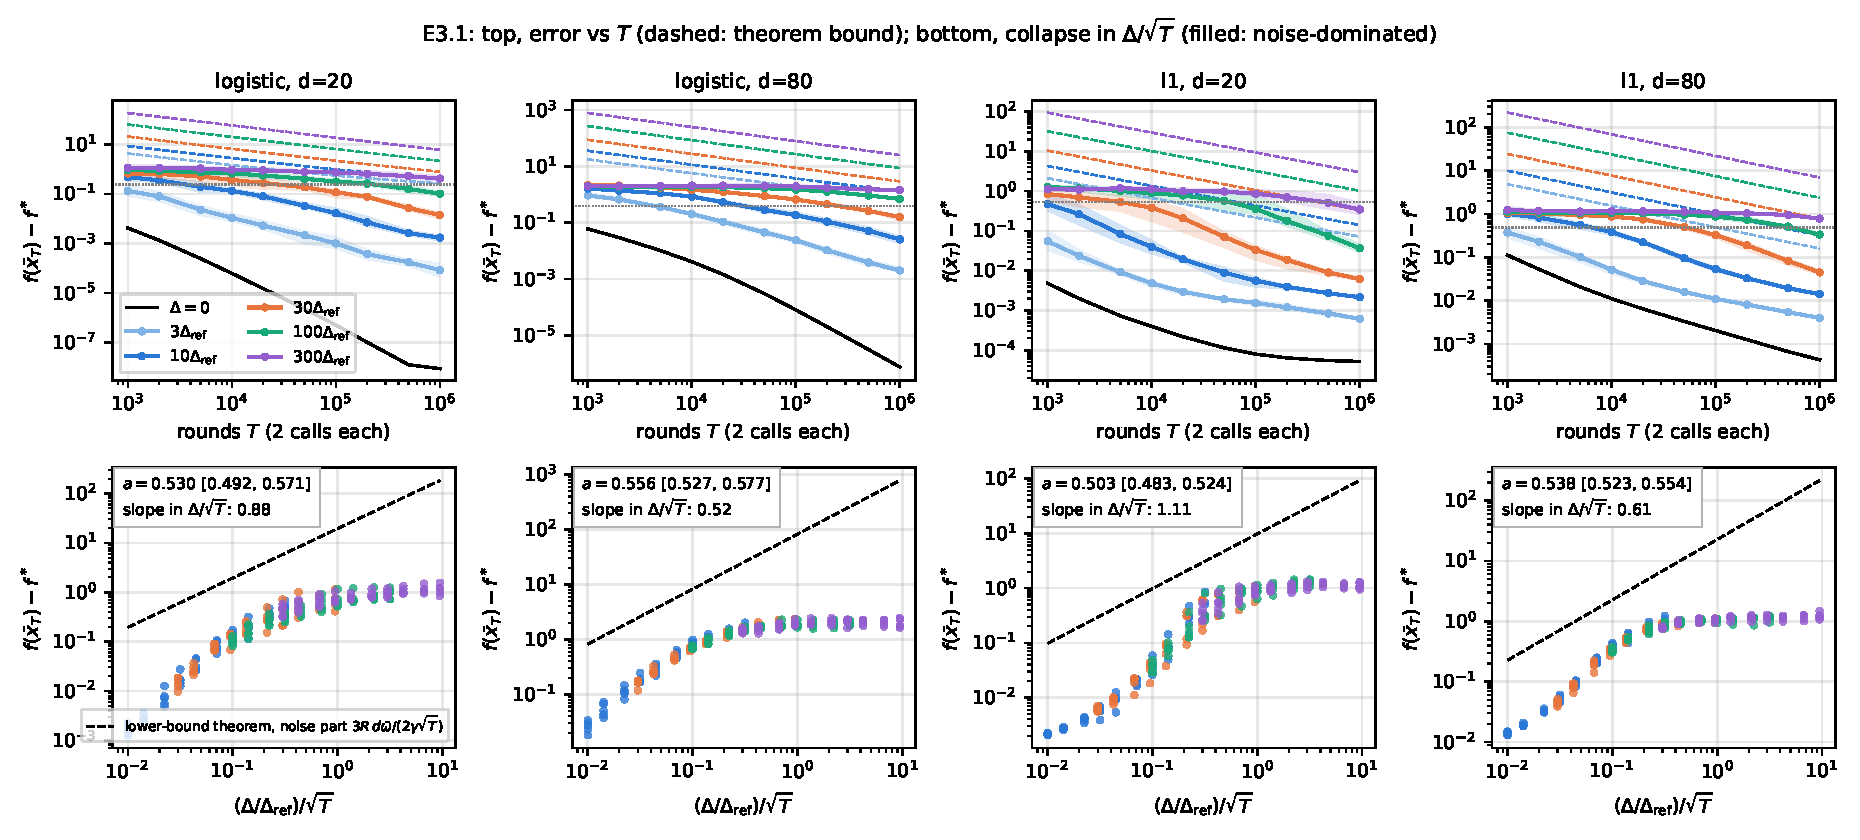
\includegraphics[width=\textwidth]{figs/e31.pdf}
\caption{E3.1. Сверху: $f(\bar x_T)-f^*$ в зависимости от числа раундов (логарифмические оси), среднее геометрическое по 5~запускам с полосой минимум--максимум; штриховая линия: оценка теоремы $3RG/\sqrt T+2M\gamma$ для каждого $\Delta$ (того же цвета); серая пунктирная: $f(0)-f^*$. Снизу: те же ошибки в зависимости от $(\Delta/\Delta_{\rm ref})/\sqrt T$; закрашенные точки~--- с преобладанием шума; штриховая линия: шумовая часть оценки.}\label{fig:e31}
\end{figure}

\textbf{Результат.}
\begin{center}\small\setlength{\tabcolsep}{4.5pt}
\begin{tabular}{@{}lccccc@{}}
\toprule
задача & \begin{tabular}[b]{@{}c@{}}$a$ (все,\\ 95\% ДИ)\end{tabular} & $\alpha$ & $R^2$ & \begin{tabular}[b]{@{}c@{}}$a$ (только с продвижением,\\ 95\% ДИ)\end{tabular} & \begin{tabular}[b]{@{}c@{}}макс.\ отношение\\ ошибка/оценка\end{tabular}\\
\midrule
логистическая, $d=20$ & $0.530\ [0.492,0.571]$ & $0.88$ & $0.82$ & $0.524\ [0.476,0.588]$ & $0.107$\\
логистическая, $d=80$ & $0.556\ [0.527,0.577]$ & $0.52$ & $0.73$ & $0.521\ [0.476,0.590]$ & $0.089$\\
$\ell_1$, $d=20$ & $0.503\ [0.483,0.524]$ & $1.11$ & $0.86$ & $0.492\ [0.458,0.527]$ & $0.251$\\
$\ell_1$, $d=80$ & $0.538\ [0.523,0.554]$ & $0.61$ & $0.74$ & $0.524\ [0.495,0.572]$ & $0.164$\\
\bottomrule
\end{tabular}
\end{center}
200~точек с преобладанием шума на задачу, из них $54$, $24$, $88$ и $43$ (в порядке таблицы) входят в подмножество с продвижением; медиана отношения ошибка/оценка в области преобладания шума $0.036$--$0.067$. \textbf{Вердикт.} \emph{Подмножества с продвижением:} каждый ДИ содержит $\frac12$ ($a=0.49$--$0.52$); ни один критерий не выполнен. \emph{Все точки:} критерий отчёта не выполнен (все четыре $a\in[0.50,0.56]$), но для обеих задач с $d=80$ ДИ исключает $\frac12$ (не более чем на $0.03$), что удовлетворяет критерию $a\ne\frac12$, зафиксированному до исследования. Большую часть множеств «все точки» составляют насыщенные точки при больших $\Delta/\sqrt T$, где итерация блуждает по сфере $\norm x=R-\gamma$, а ошибка перестаёт зависеть от $(\Delta,T)$; эти точки не несут информации об $a$ и доминируют в подгонках по всем точкам. Поэтому мы формулируем результат так: \textbf{совмещение по $\Delta/\sqrt T$ подтверждено численно на подмножествах с продвижением четырёх основных задач}; подгонки по всем точкам для $d=80$ исключают $\frac12$ с небольшим запасом. Локальный показатель $\alpha$ ошибки по $\Delta/\sqrt T$ не универсален ($0.5$--$1.1$ в целом, $1.3$--$2.0$ в области продвижения): кривая совмещения не является степенным законом, как и ожидалось (оценка для худшего случая: наклон 1; сильно выпуклый режим: наклон 2). Оценка выполнена всюду и консервативна примерно в $15$--$25$ раз для этих гладких или острых задач; поэтому «константа около 3.1»~--- верхняя огибающая, а не подгонка.

\textbf{Чувствительность} ($d=20$, $T\le2\cdot10^5$; рис.~\ref{fig:e31s}). Другой экземпляр логистической задачи: $a=0.560\ [0.498,0.629]$, только с продвижением $0.488\ [0.456,0.525]$. $\gamma\times2$: $0.490\ [0.453,0.531]$. $\ell_1$ с $\gamma\times5$: $0.487\ [0.444,0.515]$. Хэш-шум $\pm1$ (конструкция H3.2; наивный ZO-SGD, без декодирования): $a=0.671\ [0.558,0.832]$ при плохой подгонке ($R^2=0.56$, $\alpha=0.32$): \textbf{этот вариант удовлетворяет собственному критерию опровержения отчёта} ($a\notin[0.4,0.6]$, ДИ исключает $\frac12$); подгонка только по точкам с продвижением содержит 10~точек и непригодна. У этого варианта наибольшее $\wbar$ ($\sqrt2\Delta$ против $0.53\Delta$), а значит, наибольшая доля насыщенных точек.

\textbf{Повторный запуск при равном $\wbar$ (добавлен после первой версии этого отчёта; не слепой: эта конфигурация уже запускалась, когда записывалась её постановка).} \emph{Постановка:} вариант $\pm1$, в котором каждый уровень умножен на $\sqrt{2/7}/\sqrt2=0.378$, так что $\wbar$ равно $\wbar$ запусков с бета-шумом при номинальных уровнях; те же зёрна, что в варианте $\pm1$ (общие случайные числа), $T\le2\cdot10^5$, 5~запусков, $24$~с. \emph{Предсказание:} если аномалия вызвана насыщением, то $a\in[0.4,0.6]$ с ДИ, содержащим $\frac12$. \emph{Опровержение:} как для E3.1. \emph{Результат} (рис.~\ref{fig:e31pm1}; бутстреп с отдельным генератором): все точки $a=0.516\ [0.472,0.566]$ ($160$~точек, $\alpha=0.68$, $R^2=0.77$); подмножество с продвижением $a=0.628\ [0.516,0.772]$ ($29$~точек, $R^2=0.89$). \emph{Вердикт:} на всех точках критерий не выполнен, так что насыщение объясняет большую часть аномалии; подмножество с продвижением, при всей его малости, формально удовлетворяет критерию опровержения. Поэтому для шума $\pm1$ с наивным ZO-SGD совмещение по $\sqrt T$ \emph{не} установлено. Возможная причина, не проверявшаяся: при шуме $\pm1$ у половины пар разность шума в точности равна нулю, так что шум за раунд~--- двухточечная смесь, а не непрерывное распределение, и ошибка не обязана зависеть от $(\Delta,T)$ только через $\wbar^2/T$. Этот шум декодируем (предл.~\ref{prop:pm1}) и не используется как трудный пример.

\begin{figure}[h]\centering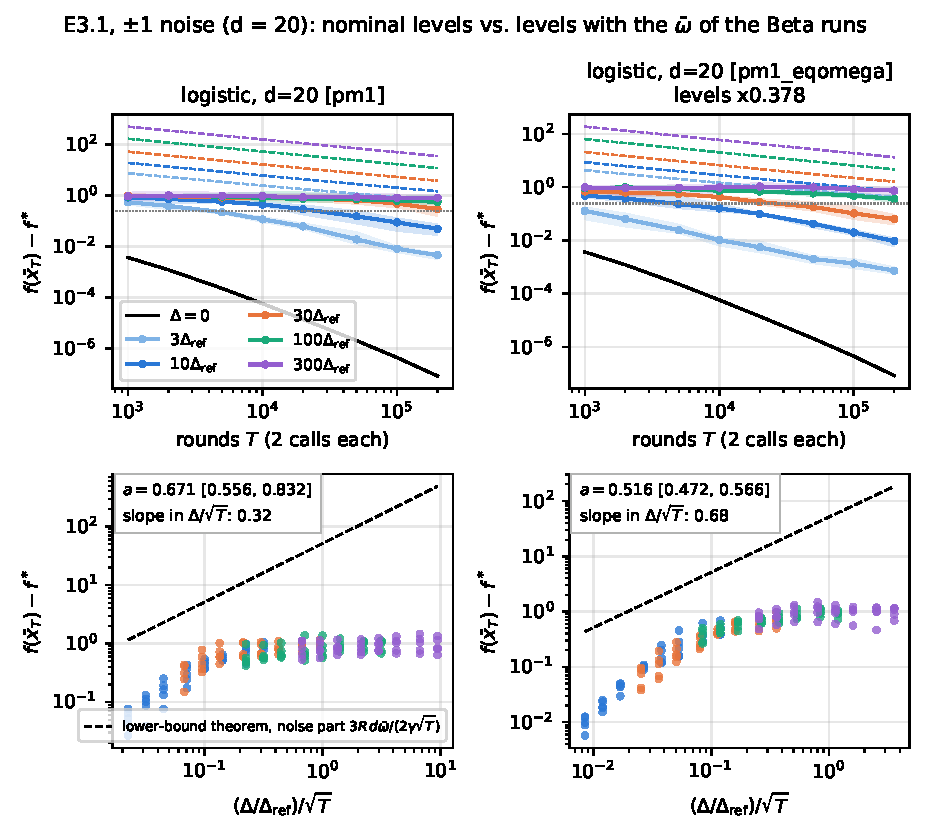
\includegraphics[width=0.62\textwidth]{figs/e31_pm1_eqomega.pdf}
\caption{E3.1, шум $\pm1$ ($d=20$, логистическая регрессия): слева~--- вариант чувствительности при номинальных уровнях; справа~--- повторный запуск при равном $\wbar$ (уровни $\times0.378$). Обозначения те же, что на рис.~\ref{fig:e31}; ось абсцисс нижнего ряда использует фактический уровень $\Delta/\Delta_{\rm ref}$, а штриховая линия использует $\wbar$ шума $\pm1$.}\label{fig:e31pm1}
\end{figure}

\begin{figure}[h]\centering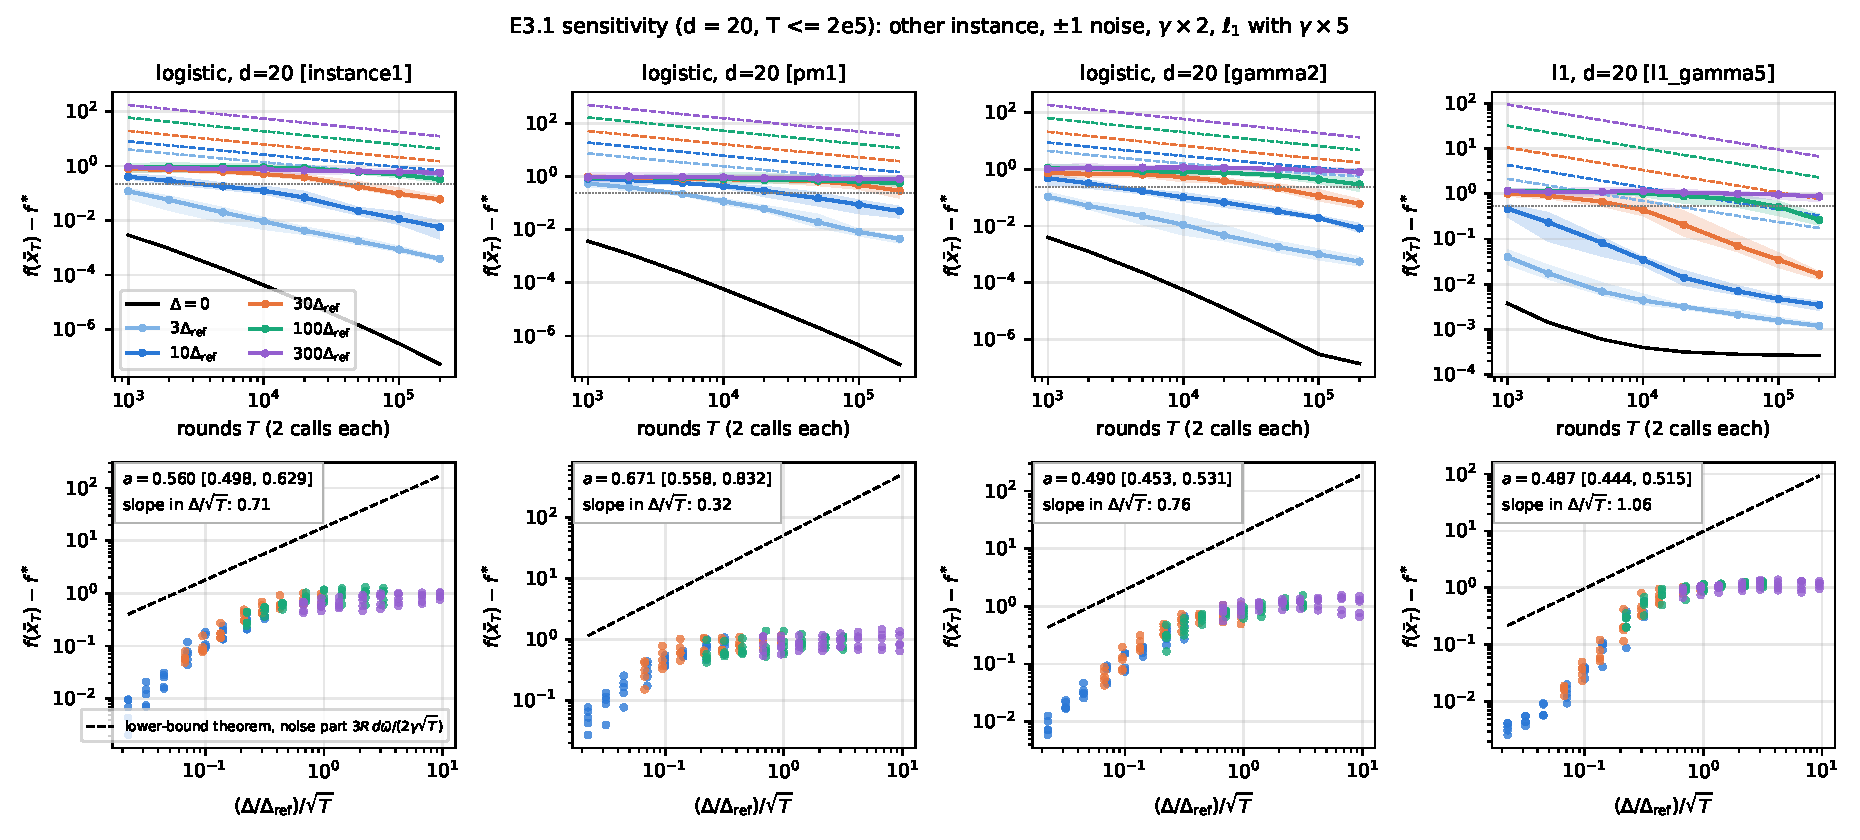
\includegraphics[width=\textwidth]{figs/e31_sensitivity.pdf}
\caption{Чувствительность E3.1: другой экземпляр, шум $\pm1$, $\gamma\times2$, $\ell_1$ с $\gamma\times5$ ($d=20$, $T\le2\cdot10^5$). Обозначения те же, что на рис.~\ref{fig:e31}; штриховая линия в нижнем ряду использует $\wbar$ каждого шума.}\label{fig:e31s}
\end{figure}

\subsection{E3.2: гладкий шум против негладкого}\label{sec:e32}
\textbf{(a) Уровень оценки.} \emph{Постановка.} $\gamma=\Delta=1$, $d\in\{20,80\}$, 28~логарифмически равномерных значений $\ell/\gamma\in[10^{-2},10^{2.5}]$, $5\times2\cdot10^5$ выборок на точку. \emph{Предсказание} (точное, без свободных параметров, лемма~\ref{lem:sin}): $\E\norm n^2/(d^2\Delta^2/4\gamma^2)=1-\Phi_d(2\gamma/\ell)$. \emph{Опровержение:} отклонения сверх погрешности МК. \emph{Результат.} Максимальное относительное отклонение $0.49\%$ ($d=20$) и $0.62\%$ ($d=80$); максимальное $\abs z=2.8$ и $3.4$ по 28~точкам в каждом случае. Второе значение пограничное для 56~тестов (объединённая стандартная ошибка среднего квадратов с тяжёлыми хвостами сама шумна); тождество, на котором основано предсказание, независимо проверено квадратурой с точностью до $10^{-14}$ (V8). \emph{Вердикт:} подтверждено. Предсказание $\min\{1,(\gamma/\ell)^2\}$ из формулировки гипотезы ошибается примерно в $d/2$ раз при $\ell\gtrsim\gamma$ (рис.~\ref{fig:e32}, слева).

\textbf{(b) Уровень оптимизации.} \emph{Постановка.} Логистическая регрессия, $\gamma=0.05$, $\Delta=30\Delta_{\rm ref}$, $T=10^5$, 5~запусков; один общий шаг (настроенный на негладкий предел $\wbar=\Delta$) для всех $\ell$; стоимость $:=$ (ошибка $-$ ошибка без шума) / (то же при $\ell=0.01\gamma$). \emph{Предсказание:} стоимость $\approx1-\Phi_d(2\gamma/\ell)$ с точностью до множителя 2 там, где она $\ge0.05$. \emph{Опровержение (формулировка гипотезы):} стоимость не зависит от $\ell$.
\begin{center}\footnotesize\setlength{\tabcolsep}{3pt}
\begin{tabular}{@{}lccccc@{}}
\toprule
$\ell/\gamma$ & $0.1$ & $0.3$ & $1$ & $3$ & $\ge10$\\
\midrule
$d=20$: измерено [ДИ] & $1.32\ [1.08,1.64]$ & $0.73\ [0.68,0.80]$ & $0.18\ [0.12,0.23]$ & $0.019\ [0.009,0.031]$ & $\le0.002$\\
\quad теория $1-\Phi_{20}$ & $1.00$ & $0.69$ & $0.096$ & $0.011$ & $\le0.001$\\
$d=80$: измерено [ДИ] & $1.12\ [1.08,1.16]$ & $0.77\ [0.67,0.87]$ & $0.068\ [0.054,0.081]$ & $0.004\ [0.000,0.009]$ & $\le0.001$\\
\quad теория $1-\Phi_{80}$ & $0.92$ & $0.24$ & $0.025$ & $0.003$ & $0.000$\\
\bottomrule
\end{tabular}
\end{center}
\emph{Вердикт.} Критерий опровержения из формулировки гипотезы не выполнен: стоимость падает на три порядка между $\ell=0.1\gamma$ и $\ell=10\gamma$. При $\ell=\gamma$ измеренная стоимость равна $0.18$ ($d=20$) и $0.068$ ($d=80$) против $1$, предсказанной $\min\{1,(\gamma/\ell)^2\}$: это предсказание опровергнуто. Заранее зафиксированное согласие с $1-\Phi_d$ с точностью до множителя 2 выполнено для $d=20$ (худшее отношение $1.9$ при $\ell=\gamma$), но нарушено для $d=80$ при $\ell=0.3\gamma$ ($\times3.2$) и $\ell=\gamma$ ($\times2.8$). По крайней мере частично это объясняется недостатком дизайна: при $\Delta=30\Delta_{\rm ref}$, $T=10^5$ ошибка в негладком пределе насыщена ($1.08$ против $f(0)-f^*=0.40$ при $d=80$; $0.258$ против $0.241$ при $d=20$), так что избыточные ошибки сжаты к опорному значению, и отношение не пропорционально избыточному второму моменту. Второй, необъяснённый признак указывает в ту же сторону: при $\ell=0.1\gamma$ нормированная стоимость превышает $1$, и ДИ исключают $1$ ($1.32\ [1.08,1.64]$ при $d=20$, $1.12\ [1.08,1.16]$ при $d=80$), тогда как теория второго момента даёт $1.00$ и $0.92$. Итак, в этом дизайне избыточная ошибка оптимизации не является функцией только избыточного второго момента $\E\norm n^2$; почему, мы не исследовали. Чистым тестом является закон на уровне оценки (a); положение излома на уровне оптимизации для $d=80$ остаётся открытым. Побочный результат: хэш-шум с бета-распределением и тем же $\wbar$, что у негладкой синусоиды, даёт ту же ошибку ($0.255$ против $0.258$ при $d=20$; $1.23$ против $1.08$ при $d=80$), что согласуется с тем, что существенный параметр~--- $\wbar$ (следствие~\ref{cor:osc}).
\begin{figure}[h]\centering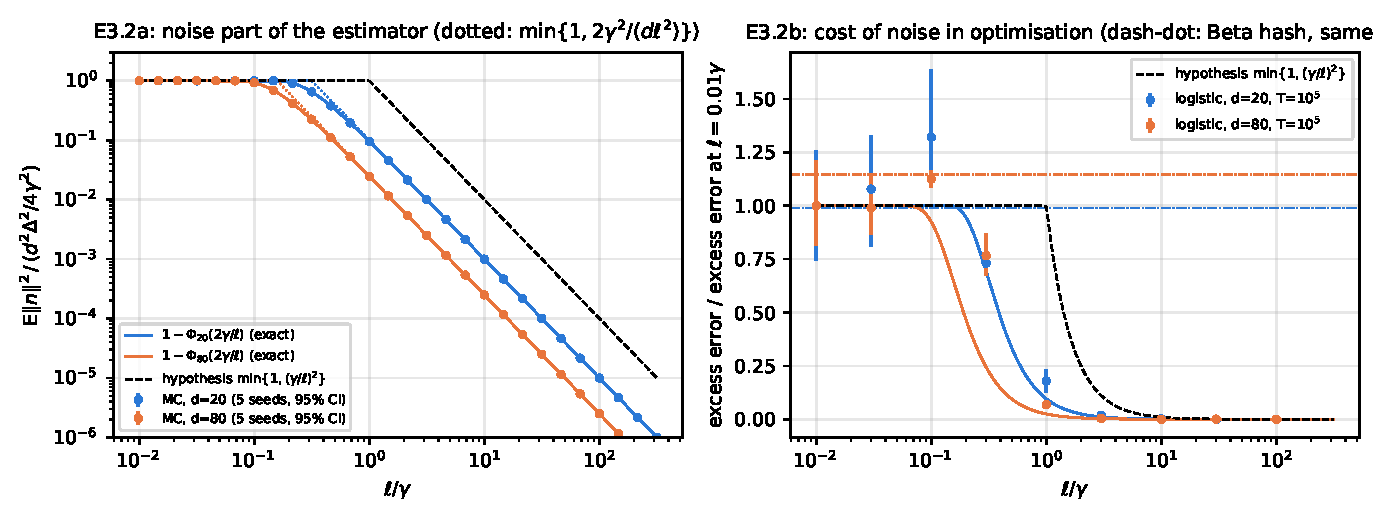
\includegraphics[width=\textwidth]{figs/e32.pdf}
\caption{E3.2. Слева: нормированное $\E\norm n^2$ в зависимости от $\ell/\gamma$ (логарифмические оси); точки: МК с 95-процентным ДИ; сплошная линия: точное $1-\Phi_d(2\gamma/\ell)$; пунктир: $\min\{1,2\gamma^2/(d\ell^2)\}$; чёрная штриховая: гипотеза $\min\{1,(\gamma/\ell)^2\}$. Справа: избыточная ошибка оптимизации, нормированная при $\ell=0.01\gamma$ (среднее, 95-процентный бутстреп-ДИ по запускам); сплошная линия: $1-\Phi_d$; штрихпунктир: хэш-шум с бета-распределением и тем же $\wbar$.}\label{fig:e32}
\end{figure}

\subsection{E3.3: одноточечные методы против двухточечных (не запускался)}\label{sec:e33}
Честная проверка требует реализации ядерного одноточечного метода (Lattimore--Gy\"orgy; Fokkema et al.); в доступные ресурсы это не уместилось. Что сделано вместо этого: (i)~строгие составляющие~--- предл.~\ref{prop:any}, \ref{prop:ballavg} и следствие~\ref{cor:cross}; (ii)~аналитическое сравнение на рис.~\ref{fig:e33}, где изображены доказанная двухточечная вилка, бандитная формула $d^{-k/2}$ (с $C_b=1$, это предположение) и универсальная верхняя оценка в единицах $\varepsilon\sqrt T$. Бандитные кривые~--- нормированная на размах гарантия $\Delta_{\rm band}(T)$ из следствия~\ref{cor:cross}, построенная при бюджетах $T=64\,d^k(MR/\varepsilon)^2$ и $256\,d^k(MR/\varepsilon)^2$ (т.\,е.\ $64d^{k-1}T_0$ и $256d^{k-1}T_0$; $C_b=1$); при $T\le16d^{k-1}T_0$, что включает каждый бюджет, сохраняющий сложность, $CT_0$ с $C\le16d^{k-1}$, они тождественно равны нулю. При $C_b=1$ пересечение (crossover) с двухточечной верхней оценкой для $d=20$, $k=3$ находится при $MR/\varepsilon\approx128\pi\sqrt{20}\approx1.8\cdot10^3$ для большего бюджета, а не при $\sqrt d$; поэтому положение пересечения~--- утверждение о константах, которые никто не вычислял. \textbf{План запуска.} Реализовать одноточечный ядерный метод Lattimore--Gy\"orgy 2023 (или более простой эллипсоидный вариант Fokkema et al.\ 2024) с усреднением по шару (предл.~\ref{prop:ballavg}); квадратичная и $\ell_1$ целевые функции, $d\in\{10,20,40\}$, $MR/\varepsilon\in\{2,5,10,30,100\}$, клеточный шум из опр.~\ref{def:noise} при $\Delta\in\{10,30,100\}\Delta_{\rm ref}$; измерить $\Delta_{50}(T)$ для обоих методов и точку пересечения по $MR/\varepsilon$. Опровержение, как зафиксировано заранее: пересечения нет.
\begin{figure}[h]\centering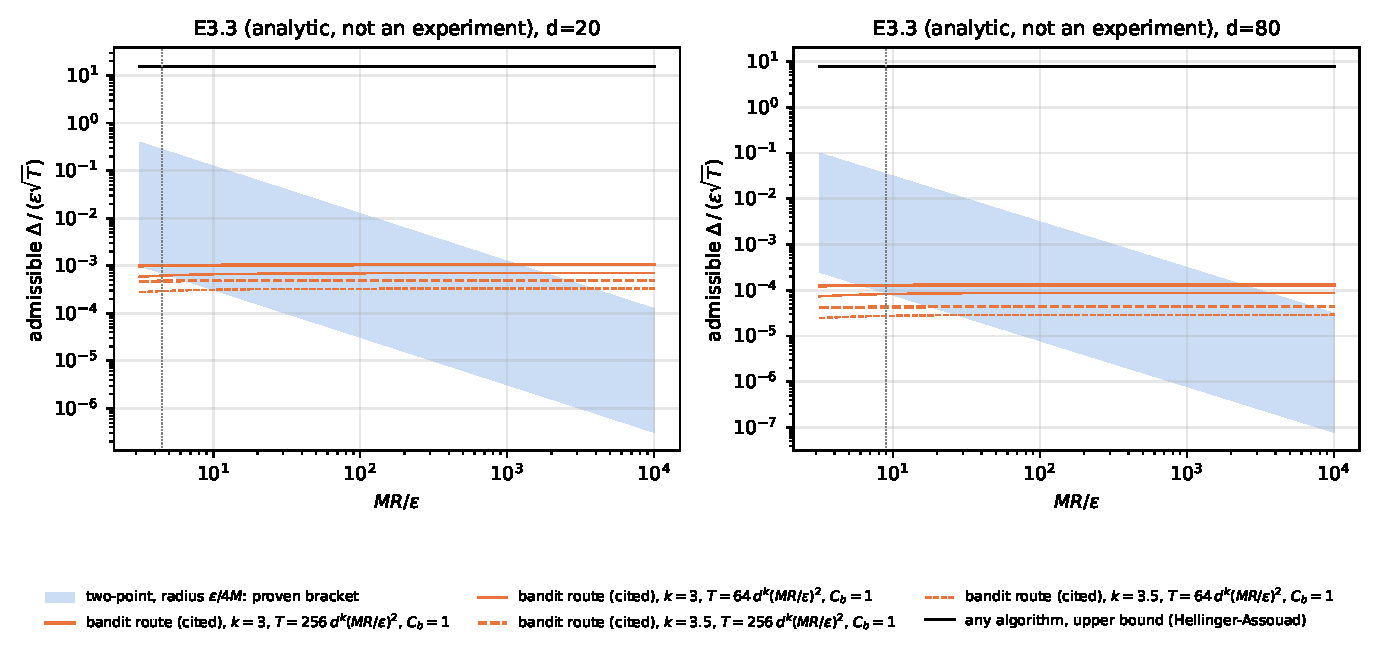
\includegraphics[width=\textwidth]{figs/e33_analytic.pdf}
\caption{E3.3 (аналитика, не эксперимент). Допустимое $\Delta/(\varepsilon\sqrt T)$ в зависимости от $MR/\varepsilon$ при $\gamma=\varepsilon/(4M)$. Синяя полоса: доказанная вилка для $\Atwo$ (теор.~\ref{thm:main}); оранжевые: нормированная на размах бандитная гарантия $\Delta_{\rm band}$ из следствия~\ref{cor:cross} при $T=256\,d^k(MR/\varepsilon)^2$ (толстая) и $64\,d^k(MR/\varepsilon)^2$ (тонкая), $C_b=1$, цитируемые скорости не перепроверены; она обращается в нуль при $T\le16d^k(MR/\varepsilon)^2$; чёрная: верхняя оценка для любого алгоритма (предл.~\ref{prop:any}); пунктир: $MR/\varepsilon=\sqrt d$.}\label{fig:e33}
\end{figure}

\subsection{E3.4 (новый): трудный пример против ZO-SGD}\label{sec:e34}
\textbf{Постановка.} $f_v=a\ip vx$ на $B_1$, хэш-шум с бета-распределением ($I=10$), $\Delta=1$, $\gamma=0.01$, $d\in\{20,80\}$, $T\in\{10^3,10^4,10^5\}$, $a=a^*\times\{\frac1{16},\frac14,1,4,16\}$ с $a^*=\sqrt d\Delta/(4\gamma\sqrt{IT})$; 20~запусков (5~зёрен $\times$ 4~случайных $v$) на ячейку; масштаб шага $\in\{0.1,1,10\}$, приводится лучший (каждый масштаб шага~--- отдельный алгоритм из $\Atwo$, так что минимум их рисков по-прежнему ограничен снизу). \textbf{Предсказание.} Лемма~\ref{lem:assouad} с оценками теор.~\ref{thm:upper}: средняя ошибка $\ge LB(a)=\frac{aR}{4\sqrt d}(d-2\gamma a\sqrt{dIT}/\Delta)_+$. \textbf{Опровержение.} Средняя ошибка (верхний конец её 95-процентного ДИ) ниже $LB$. \textbf{Результат.} Опровержения нет ни разу: наименьшее отношение (нижний конец ДИ)$/LB$ равно $3.7$; при $a=a^*$ отношение составляет $5.9$--$6.6$ во всех шести ячейках $(d,T)$. В единицах $a^*R\sqrt d$ кривые для разных $T$ совпадают (рис.~\ref{fig:e34}), как и предсказывает масштабирование $a^*\propto\sqrt d\Delta/(\gamma\sqrt T)$. \textbf{Вердикт: только проверка на здравый смысл.} Тест не может провалиться для метода, который ничему не учится, поскольку $LB(a)\le aR\sqrt d/4$ меньше тривиальной ошибки $aR\sqrt d$ выхода $\hat x=0$; и действительно, при $a\le a^*$ ZO-SGD остаётся на уровне $0.79$--$1.00$ от тривиальной ошибки. Отношение $\approx6$ при $a^*$ отражает множитель $\frac18$ оценки Ассуада относительно тривиальной ошибки, а не близость $32\pi$ к точности. ZO-SGD достигает относительной точности $\frac18$, которую оценка гарантирует при $a^*$, лишь около $a\approx16a^*$ (ошибка/тривиальная $0.11$--$0.18$). E3.4 не засчитывается как подтверждение H3.2a.
\begin{figure}[h]\centering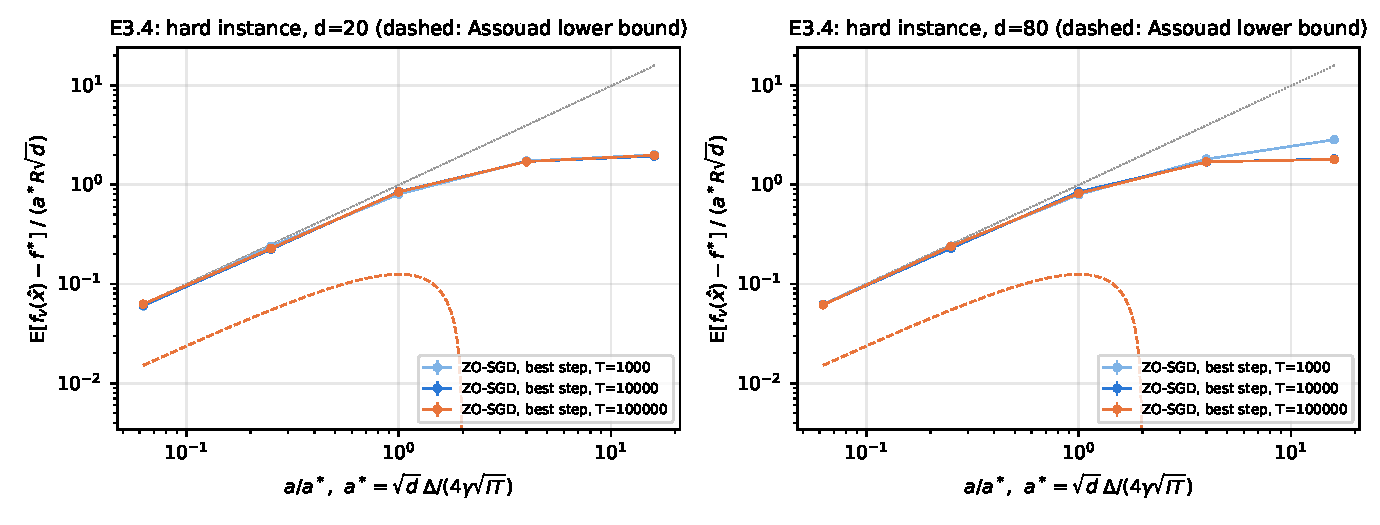
\includegraphics[width=\textwidth]{figs/e34.pdf}
\caption{E3.4. Средняя ошибка ZO-SGD (лучший из 3~шагов; 95-процентный ДИ по 20~запускам) на трудном примере в зависимости от $a/a^*$, в единицах $a^*R\sqrt d$; штриховая линия: нижняя оценка Ассуада (она обращается в нуль при $a\ge2a^*$, где ограничение по константе Липшица не активно); пунктир: прямая $y=x$, тривиальная ошибка начальной точки $\hat x=0$.}\label{fig:e34}
\end{figure}

\subsection{E3.5 (новый): шум $\pm1$ декодируем}\label{sec:e35}
\textbf{Постановка.} Логистическая регрессия, $d=20$, $\gamma=0.05$, $\Delta/\Delta_{\rm ref}\in\{10,100\}$ (здесь $2M\gamma=8.94\Delta_{\rm ref}$), $T=10^5$, 5~запусков; ветви: без шума; хэш-шум $\pm1$, декодированный по $g=D-2\Delta\,\mathrm{round}(D/2\Delta)$ (тот же поток направлений, что и в ветви без шума); $\pm1$ без декодирования; бета-шум без декодирования с тем же $\Delta$. \textbf{Предсказание} (предл.~\ref{prop:pm1}): декодированная ветвь $=$ ветвь без шума с точностью до ошибки округления. \textbf{Результат.} Максимальная разность записанных ошибок $1.7\cdot10^{-16}$; итоговые ошибки: без шума и с декодированием $4.2\cdot10^{-7}$; $\pm1$ без декодирования: $0.10$ и $0.79$; бета-шум без декодирования: $0.014$ и $0.46$. \textbf{Вердикт.} Подтверждено. Конструкция H3.2 в исходном виде побеждает ZO-SGD, но при $\Delta>2M\gamma$~--- не алгоритм того же класса с одной дополнительной строкой; поэтому наша верхняя оценка использует вместо неё распределение с конечной информацией Фишера (необходимо ли такое распределение при $\Delta\le2M\gamma$, не показано).
\begin{figure}[h]\centering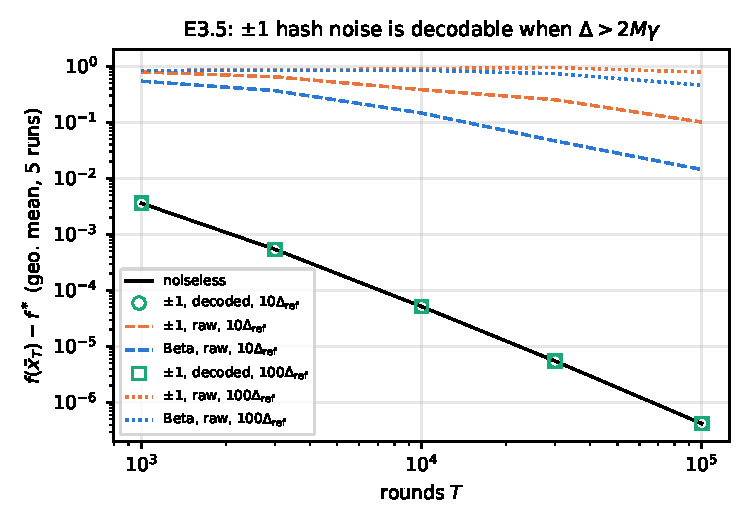
\includegraphics[width=0.62\textwidth]{figs/e35.pdf}
\caption{E3.5. Ошибка в зависимости от числа раундов (среднее геометрическое по 5~запускам). Полые маркеры (декодированный шум $\pm1$) лежат точно на кривой без шума.}\label{fig:e35}
\end{figure}

%==========================================================================================
\section{Вердикт}\label{sec:verdict}
{\small
\begin{xltabular}{\textwidth}{@{}>{\raggedright\arraybackslash}p{5.3cm}>{\raggedright\arraybackslash}p{4.6cm}>{\raggedright\arraybackslash}X@{}}
\toprule
Утверждение & Статус & На что опирается\\
\midrule
\endhead
H3.1a ZO-SGD (пакет размера 1, холостой раунд~1) имеет точность $\varepsilon$ при $\wbar/2\le\Dlow(T)$, явные константы & доказано при условии (независимые одинаково распределённые состояния с произвольным начальным распределением, один холостой раунд~--- или стационарный старт без него; выпуклая $M$-липшицева $f$, $\gamma+\rho\le\varepsilon/(4M)$; вариант «в~среднем»; «по~вероятности» с заменой $\varepsilon\to\beta\varepsilon$) & лемма~\ref{lem:mom}, теор.~\ref{thm:lower}, следствие~\ref{cor:lower}, замечание~\ref{rem:lower}(vi); V11, V17; E3.1 (оценка выполнена, макс.\ отношение 0.25)\\
H3.1b $\Dcp^E(24)\ge1.034M\gamma/\sqrt d$ при $\tau=1$ (вариант «в~среднем»; вариант «по~вероятности» при $C=24/\beta^2$) & доказано (те же условия, $\varepsilon<MR/8$) & следствие~\ref{cor:lower}(b); V15\\
H3.1c согласованность с эвристическим порогом ($\xi\equiv0$, $b=1$ даёт $M\gamma/\sqrt d$) & проверка согласованности (неформальная) & замечание~\ref{rem:lower}(i)\\
H3.2a $\Dmax^{E,\mathrm{2pt},\gamma}\le32\pi\varepsilon\gamma\sqrt T/(dR)$ & доказано для $\Atwo$ (неадаптивные распределения направлений), $\varepsilon<MR/8$ & леммы~\ref{lem:inclass}--\ref{lem:couple}, теор.~\ref{thm:upper}; V1, V3--V7 (E3.4~--- только проверка на здравый смысл)\\
H3.2b то же для адаптивных распределений направлений & остаётся гипотезой & замечание~\ref{rem:scope}(i)\\
H3.2c двусторонняя оценка $\Theta(\varepsilon\gamma\sqrt T/(dR))$ & доказано для $\Atwo$ при условиях теор.~\ref{thm:main} (выпуклая $M$-липшицева $f$, $\gamma\le\varepsilon/(4M)$; гладкий класс с $\gamma>\varepsilon/(4M)$ не покрыт) & теор.~\ref{thm:main}, замечание~\ref{rem:scope}(iv); E3.1 (совмещение на подмножествах с продвижением)\\
H3.2d клеточный шум $\pm1$ даёт верхнюю оценку & опровергнуто при $\Delta>2M\gamma$ (любая $f$) и для семейства линейного гиперкуба при любом $\Delta$; открыто для других семейств при $\Delta\le2M\gamma$ & предл.~\ref{prop:pm1}; V13; E3.5\\
H3.3a любой алгоритм: $\Dmax^E\le16\sqrt2\pi\varepsilon\sqrt T/\sqrt d$ & доказано & предл.~\ref{prop:any}\\
H3.3b бандитные методы лучше двухточечных при $MR/\varepsilon\gtrsim\sqrt d$ & доказано при условии: предположение (B$_k$) (цитируемые скорости для потерь в $[0,1]$, не перепроверены, $C_b$ неизвестна), бюджет $T\ge2+256C_bd^{k-1}T_0$ и $MR/\varepsilon>128\pi\sqrt{C_b}d^{k/2-1}$ ($\sqrt d$ при $k=3$, $d^{3/4}$ при $k=3.5$) & следствие~\ref{cor:cross}; V16; E3.3 не запускался. При $T\le2+16C_bd^{k-1}T_0$ (каждый бюджет, сохраняющий сложность, $CT_0$ с $C\le16C_bd^{k-1}$) цитируемые скорости не дают гарантии\\
H3.3c фиксированный $\gamma$: бесселева часть блокирует бандитные методы & опровергнуто (информационно-теоретически) & предл.~\ref{prop:ballavg}\\
H3.3d класс всех радиусов: истинный порог $=$ максимум двух формул & остаётся гипотезой (нижняя сторона условна, разрыв сверху $d^{(k-1)/2}$) & следствие~\ref{cor:cross}\\
H3.4a шумовая часть $\le d\omega_\delta/(2\gamma)$; оценки через $\omega_\delta/2$ и $\wbar/2$ & доказано & лемма~\ref{lem:osc}, следствие~\ref{cor:osc}\\
H3.4b $\Lambda$-липшицев шум стоит $M\to M+\Lambda$ & доказано & следствие~\ref{cor:lip}; V12\\
H3.4c гладкий шум: стоимость $\propto1-\Phi_d(2\gamma/\ell)$, излом при $\gamma/\sqrt d$ (уточняет «$\min\{1,\gamma/\ell\}^2$») & доказано (для оценки); подтверждено численно (E3.2a); уровень оптимизации: подтверждено для $d=20$, не для $d=80$ & лемма~\ref{lem:sin}; V8; E3.2\\
H3.4d округление: $\omega_\delta\le u$, $\wbar\le u/2$, совпадение $=$ стёртый сигнал & доказано (только для равномерного свежего сдвига) & предл.~\ref{prop:round}; V10\\
E3.1 совмещение по $\Delta/\sqrt T$ & подтверждено численно на подмножествах с продвижением четырёх основных задач; подгонки по всем точкам для $d=80$ исключают $\frac12$ (на $\le0.03$); вариант $\pm1$ удовлетворяет критерию опровержения, что в основном объясняется насыщением (повторный запуск при равном $\wbar$), подмножество с продвижением в повторном запуске по-прежнему аномально & \S\ref{sec:e31}; рис.~\ref{fig:e31pm1}\\
Замечание о $T\ll T_0$ и второй ветви H2 (более ранняя версия этого отчёта: «$\Delta=0$ неразрешимо, ветвь пуста») & отозвано (ссылка неприменима) & замечание~\ref{rem:scope}(iii)\\
\bottomrule
\end{xltabular}}

%==========================================================================================
\section{Следствия}\label{sec:contrib}
\subsection{Для общей задачи}
\begin{enumerate}
\item Ожидаемая картина $\Delta^{\rm adv}_{\max}\lesssim\Dcp(C)\lesssim M\gamma/\sqrt d$ теперь доказана с обеих сторон при $\tau=1$ \emph{для двухточечных методов радиуса $\gamma$} и выпуклых $M$-липшицевых $f$ с $\gamma\le\varepsilon/(4M)$. Два отдельных утверждения: \emph{нижняя сторона} (следствие~\ref{cor:lower}(b), доказано) $\Dcp^{E,\mathrm{2pt},\gamma}(24)\ge1.034M\gamma/\sqrt d$ в варианте «в~среднем» и $\Dcp(24/\beta^2)\ge1.034M\gamma/\sqrt d$ в варианте «по~вероятности»; \emph{верхняя сторона} (теор.~\ref{thm:upper}, доказано для $\Atwo$) при $T=CT_0=CdM^2R^2/\varepsilon^2$: $\Dcp^{E,\mathrm{2pt},\gamma}(C)\le32\pi\,\varepsilon\gamma\sqrt{CT_0}/(dR)=32\pi\sqrt C\,M\gamma/\sqrt d$ при $\varepsilon<MR/8$ и $\Dcp^{\mathrm{2pt},\gamma}(C)\le64\pi\sqrt C\,M\gamma/\sqrt d$ в варианте «по~вероятности» при $\beta\le1/32$, $\varepsilon<MR/16$. Именно верхняя сторона закрывает H1.5d для $\tau=1$ и $\Atwo$.
\item Для произвольных точек запроса наши оценки порог не характеризуют: они оставляют разрыв до $\asymp\sqrt d\,MR/\varepsilon$ между $\Dlow$ и $71\varepsilon\sqrt T/\sqrt d$ (предл.~\ref{prop:any}, доказано). Цитируемые бандитные скорости после перенормировки на размах $f$ превосходят двухточечную верхнюю оценку лишь при бюджетах $T\gtrsim C_bd^{k-1}T_0$ и при $MR/\varepsilon\gtrsim d^{k/2-1}$ (доказано при предположении (B$_k$)); при бюджетах, сохраняющих сложность, $T\asymp CT_0$ они не дают гарантии и не превосходят двухточечные методы (следствие~\ref{cor:cross}). Поэтому значение $\Dmax$ зависит от того, к какому классу алгоритмов оно относится: для $\Atwo$ при $\tau=1$ и условиях теор.~\ref{thm:main} (выпуклая $M$-липшицева $f$ на $B_R$, произвольное начальное распределение, $\varepsilon<MR/8$, $\gamma\le\varepsilon/(4M)$, $T\ge1+16d^2M^2R^2/((d-1)\varepsilon^2)$) оно равно $\Theta(\varepsilon\gamma\sqrt T/(dR))$; для всех алгоритмов оно лишь заключено в вилку.
\item Параметр шума двухточечной задачи~--- (среднеквадратичное) колебание на масштабе $2\gamma$, а не амплитуда: в каждой оценке этого отчёта для двухточечных методов $\Delta$ можно заменить на $\omega_\delta(2\gamma)/2$ (следствие~\ref{cor:osc}, доказано).
\end{enumerate}

\subsection{Для других гипотез}
\textbf{H2:} первая ветвь при $\tau=1$ доказана с обеих сторон для $\Atwo$ (в H1 она была доказана только снизу, с прогревом); о второй ветви $\sqrt{\ln T/d}$ ничего не выводится (замечание~\ref{rem:scope}(iii)). \textbf{H5:} ожидается, что аппарат верхних оценок (расстояние Хеллингера, последовательная оценка BC, каплинг с идеализированным оракулом) применим к конструкции с ложными долинами (здесь не проверялось); урок шума $\pm1$ применим и к H5.1--5.2: двузначный шум внутри состояния может быть декодируемым (по крайней мере при $\Delta>2M\gamma$, предл.~\ref{prop:pm1}), так что наша техника дала бы антисостояниям распределение шума с конечной информацией Фишера. \textbf{H4:} её базовый случай $\tau=1$~--- теор.~\ref{thm:lower}. \textbf{H6:} без изменений; предл.~\ref{prop:ballavg} показывает, что \emph{любой} алгоритм может нейтрализовать бесселеву часть усреднением по радиусу класса, так что H6~--- утверждение о методах, которые не могут (или не делают) этого. \textbf{H7, H10:} округление со свежим сдвигом~--- шум с $\tau=1$ и $\wbar\le u/2$ (предл.~\ref{prop:round}, доказано для равномерного свежего сдвига); общий дизеринг H10~--- в точности этот режим. Округление со сдвигом, управляемым методом (H8), не покрывается.

\subsection{Открытые вопросы}
\begin{enumerate}
\item \emph{Класс алгоритмов.} Больше ли при $\tau=1$ и $T\asymp CT_0$ порог для алгоритмов с произвольными точками запроса и отдельными значениями, чем порог двухточечных методов? Наша вилка там~--- $[\Dlow,\,71\varepsilon\sqrt T/\sqrt d]$.
\item \emph{Адаптивные распределения направлений.} Распространяется ли теор.~\ref{thm:upper} на методы, выбирающие распределение направлений адаптивно (H3.2b, остаётся гипотезой)?
\item \emph{Константы и область применимости.} Две стороны различаются множителем $128\pi$; нижняя сторона не покрывает гладкий класс с $\varepsilon/(4M)<\gamma\le\sqrt{\varepsilon/L}$.
\item \emph{Двузначный шум.} Является ли какой-либо двузначный шум трудным на уровнях, сохраняющих сложность, $\Delta\lesssim\sqrt C M\gamma/\sqrt d<2M\gamma$, или распределение с конечной информацией Фишера необходимо?
\item \emph{Численные эксперименты.} E3.3 (одноточечные методы против двухточечных) не запускался; излом на уровне оптимизации в E3.2 для $d=80$ и остаточная аномалия шума $\pm1$ на подмножестве с продвижением в повторном запуске при равном $\wbar$ не объяснены.
\end{enumerate}

%==========================================================================================
\appendix
\section{Проверки}\label{app:checks}
\begin{center}\small
\begin{tabularx}{\textwidth}{@{}lXl@{}}
\toprule
ID & Проверка & Результат\\
\midrule
V1 & информация Фишера и нормировка: $I(\cos^2(\pi t/2))=\pi^2$, $I(\frac{15}{16}(1-t^2)^2)=10$ (sympy) & точно\\
V2 & $\mathrm{Var}=\frac13-\frac2{\pi^2}$ и $\frac17$ (sympy) & точно\\
V3 & $H^2(p_b,p)\le b^2I/4$, обе плотности, $b\in[10^{-3},1]$ (квадратура) & макс.\ отношение $0.9997$\\
V4 & то же для распределения $U-U'$ (бета-случай; обработка данных) & отношения $0.34$--$0.36$\\
V5 & хэш-шум: критерий Колмогорова--Смирнова против $\mathrm{Beta}(3,3)$, независимость пары, ни одной пары в одной клетке ($10^5$ пар) & $p=0.07$, корр.\ $7.7\cdot10^{-4}$, 0~пар\\
V6 & $\sqrt d-\sqrt{d-i}\ge i/(2\sqrt d)$ ($d<400$); лемма о разделении на случайных точках & пройдена, мин.\ запас $4\cdot10^{-10}$\\
V7 & последовательная оценка BC и $\TV\le\sqrt{1-\BC^2}$, 200~случайных адаптивных двухраундовых схем (точно) & пройдена\\
V8 & $\E\sin^2(\kappa e_1)=\frac12(1-\Phi_d(2\kappa))$, $d\in\{3,20,80\}$ & погрешность $10^{-14}$\\
V9 & $\sqrt6-\sqrt{d/(d-1)}\ge1$ при $2\le d\le10^4$; константы $32\pi$, $32\sqrt{10}$, $16\sqrt2\pi$ & мин.\ $1.035$\\
V10 & округление с равномерным сдвигом: закон совпадений, $\E(D\delta)^2=u^2r'(1-r')$, $\abs{D\delta}\le u$ & пройдена ($4\cdot10^5$ выборок)\\
V11 & $\E\norm Y^2\le G^2$ (логистическая регрессия, бета-шум, $\Delta=30\Delta_{\rm ref}$) & отношение $0.79$\\
V12 & оценка для липшицева шума $d^2(M+\Lambda)^2/(d-1)$ & $51\le276$\\
V13 & декодер $\pm1$ точен при $\abs g<\Delta$ & пройдена\\
V14 & $I(U-U')\le I(U)$ (бета) & $3.63\le10$\\
V15 & следствие~\ref{cor:lower}(b) с холостым раундом: $\varepsilon\sqrt{24T_0-1}/(2R)=\sqrt dM\sqrt{6(1-1/(24T_0))}$ (sympy); множитель $\ge1.034$ при $T_0>64d$, $2\le d\le10^4$ & мин.\ $1.0349$ ($d=2$)\\
V16 & следствие~\ref{cor:cross}: $\Delta_{\rm band}$, найденное из бюджета (sympy); оба пересечения; чистая форма (b) на сетке & пройдена\\
V17 & смещение в раунде~1 из замечания~\ref{rem:lower}(vi), $d\in\{20,80\}$, $2\cdot10^5$ выборок, против $\frac d\gamma\Delta\E\abs{e_1}$ & в пределах $4$ ст.\ ош.\\
\bottomrule
\end{tabularx}
\end{center}
Проверки V1--V17 занимают около 4~с; все запуски вместе~--- около 50~мин на одном ядре CPU. Рисунки и статистика вычисляются только по сохранённым сырым результатам.

\textbf{Что не проверялось.} Цитируемые бандитные теоремы (формулировки, константы); адаптивные распределения направлений; цепи с $\tmix\le1$, не являющиеся последовательностями независимых состояний (только через H1 следствие~4.17); размерности выше $80$; E3.3; излом на уровне оптимизации в E3.2 для $d=80$ (насыщенный дизайн) и стоимости выше $1$ в E3.2b; остаточная аномалия шума $\pm1$ на подмножестве с продвижением в повторном запуске при равном $\wbar$. Воспроизводимость: при фиксированных зёрнах логистические запуски воспроизводятся с точностью до $10^{-10}$, но запуски $\ell_1$ воспроизводимы только статистически, не побитово (повторный запуск обнаружил отдельные запуски $\ell_1$ при $d=80$ на низких уровнях, отличающиеся до $42\%$, при средних геометрических по уровням в пределах примерно $10\%$; вероятная причина~--- недетерминированность вычислений с плавающей точкой в решении LP или в BLAS, усиленная негладкостью целевой функции).
\end{document}
